%Este trabalho está licenciado sob a Licença Atribuição-CompartilhaIgual 4.0 Internacional Creative Commons. Para visualizar uma cópia desta licença, visite http://creativecommons.org/licenses/by-sa/4.0/deed.pt_BR ou mande uma carta para Creative Commons, PO Box 1866, Mountain View, CA 94042, USA.

\documentclass[12pt]{book}

\input ../preambulo.tex
\input ../preambulo_python.tex

\ifispython
\lstset { %
  language=Python,
}
\fi

% \makeindex

\begin{document}

\frontmatter

\title{Matemática Numérica Avançada}
\author{Pedro H A Konzen}
\date{}
\maketitle

% ficha catolográfica
\ifisbook
~
\vspace{4.5in}
\hrule
Konzen, Pedro Henrique de Almeida\\
\indent\hspace{2em}Matemática numérica avançada: notas de aula / Pedro Henrique de Almeida Konzen. --{\the\year}. Porto Alegre.- {\the\year}.\\
\indent\hspace{2em}"Esta obra é uma edição independente feita pelo próprio autor."\\
\indent\hspace{2em}1. Métodos numéricos. 2. Análise numérica. 3. Linguagem Python.\\
\hrule
\vspace{1cm}
\begin{center}
  \textit{Licença}\\CC-BY-SA 4.0.
\end{center}
\fi

%Este trabalho está licenciado sob a Licença Atribuição-CompartilhaIgual 4.0 Internacional Creative Commons. Para visualizar uma cópia desta licença, visite http://creativecommons.org/licenses/by-sa/4.0/ ou mande uma carta para Creative Commons, PO Box 1866, Mountain View, CA 94042, USA.

\section*{Licença}\label{licenca}
\addcontentsline{toc}{section}{Licença}

Este trabalho está licenciado sob a Licença Atribuição-CompartilhaIgual 4.0 Internacional Creative Commons. Para visualizar uma cópia desta licença, visite http://creativecommons.org/licenses/by-sa/4.0/deed.pt\_BR ou mande uma carta para Creative Commons, PO Box 1866, Mountain View, CA 94042, USA.



\chapter*{Prefácio}\label{prefacio}
\addcontentsline{toc}{chapter}{Prefácio}

O site \href{https://www.notaspedrok.com.br}{notaspedrok.com.br} é uma plataforma que construí para o compartilhamento de minhas notas de aula. Essas anotações feitas como preparação de aulas é uma prática comum de professoras/es. Muitas vezes feitas a rabiscos em rascunhos com validade tão curta quanto o momento em que são concebidas, outras vezes, com capricho de um diário guardado a sete chaves. Notas de aula também são feitas por estudantes - são anotações, fotos, prints, entre outras formas de registros de partes dessas mesmas aulas. Essa dispersão de material didático sempre me intrigou e foi o que me motivou a iniciar o site.

Com início em 2018, o site contava com apenas três notas incipientes. De lá para cá, conforme fui expandido e revisando os materiais, o site foi ganhando acessos de vários locais do mundo, em especial, de países de língua portuguesa. No momento, conta com 13 notas de aula, além de minicursos e uma coleção de vídeos e áudios.

As notas de \emph{Matemática Numérica III} abordam tópicos sobre sistemas lineares de médio/grande porte, sistemas não-lineares, problemas de otimização, problemas de autovalores e integração auto-adaptativa. Códigos exemplos são apresentados em linguagem {\python}.

Aproveito para agradecer a todas/os que de forma assídua ou esporádica contribuem com correções, sugestões e críticas! ;)

\begin{flushright}
  Pedro H A Konzen

  \url{https://www.notaspedrok.com.br}
\end{flushright}

\tableofcontents
\addcontentsline{toc}{chapter}{Sumário}

\mainmatter

\chapter{Sistemas Lineares}\label{cap_sislin}
\badgeRevisar

Neste capítulo, estudamos métodos numéricos para a resolução de sistemas lineares de médio e grande porte. Salvo explicitado ao contrário, assume-se que os sistemas são quadrados e têm solução única.

\section{Matrizes Esparsas}\label{cap_sislin_sec_matesparsa}
\badgeRevisar

\hl{Uma matriz é dita ser \emph{esparsa} quando ela tem apenas poucos elementos não nulos}. A ideia é que os elementos não nulos não precisam ser guardados na memória do computador, gerando um grande benefício na redução da demanda de armazenamento de dados. O desafio está no desenvolvimento de estruturas de dados para a alocação eficiente de tais matrizes, i.e. que sejam suficientemente adequadas para os métodos numéricos conhecidos.

\begin{figure}[H]
  \centering
  \includegraphics[width=0.45\textwidth]{./cap_sislin/dados/matriz_esparsa_estruturada/main}\\
  \includegraphics[width=0.45\textwidth]{./cap_sislin/dados/matriz_esparsa_nao_estruturada/main}
  \caption{Em cima: exemplo de uma matriz esparsa estruturada. Em baixo: exemplo de uma matriz esparsa não-estruturada.}
  \label{fig:ex_matriz_esparsa_estrutura}
\end{figure}

\hl{Matrizes esparsas podem ser classificadas como \textbf{estruturadas} ou \textbf{não-estruturadas}}. Uma matriz estruturada é aquela em que as entradas não-nulas formam um padrão regular. Por exemplo, estão dispostas em poucas diagonais ou formam blocos (submatrizes densas) ao longo de sua diagonal principal. No caso de não haver um padrão regular das entradas não-nulas, a matriz esparsa é dita ser não-estruturada. Consulte a Figura \ref{fig:ex_matriz_esparsa_estrutura} para exemplos.

\hl{A \textbf{esparsidade} de uma matriz é a porcentagem de elementos nulos que ela tem}, i.e. para uma matriz quadrada $n\times n$ tem-se que a esparsidade é
\begin{equation}\hleq
  e := \frac{n_{\text{nulos}}}{n^2}\times 100\%.
\end{equation}
Por exemplo, a matriz identidade de tamanho $n=100$ tem esparsidade
\begin{equation}
  e = \frac{100^2 - 100}{100^2}\times 100\% = 99\% .
\end{equation}

\subsection{Sistemas Tridiagonais}
\badgeRevisar

Um \hlemph{sistema tridiagonal} tem a seguinte forma matricial
\begin{equation}\label{eq:sistridiag}
  \begin{bmatrix}
    a_{1,1} & {\color{violet}a_{1,2}} & & & & 0\\
    {\color{teal}a_{2,1}} & a_{2,2} & {\color{violet}a_{2,3}} & & &\\
    & {\color{teal}a_{3,2}} & a_{3,3} & {\color{violet}a_{3,4}} & &\\
    & & \ddots & \ddots & \ddots &\\
    & & & \ddots & \ddots & {\color{violet}a_{n-1,n}}\\
    0 & & & & {\color{teal}a_{n,n-1}} & a_{n,n}
  \end{bmatrix}
  \begin{bmatrix}
    x_1\\
    x_2\\
    x_3\\
    \vdots\\
    x_{n-1}\\
    x_n
  \end{bmatrix} =
    \begin{bmatrix}
    b_1\\
    b_2\\
    b_3\\
    \vdots\\
    b_{n-1}\\
    b_n
  \end{bmatrix}.
\end{equation}
Ou seja, \hl{é um sistema cuja a matriz dos coeficientes é tridiagonal}.

\hl{Uma \emph{matriz tridiagonal} é uma matriz esparsa estruturada}. Mais especificamente, é um caso particular de uma \hlemph{matriz banda}, em que os elementos não nulos estão dispostos apenas em algumas de suas diagonais. Para armazenarmos tal matriz precisamos alocar apenas os seguintes três vetores
\begin{align}
  & {\color{violet}d_{1} = \left(0,a_{1,2},\dotsc,a_{n-1,n}\right)},\\
  & d_{0} = \left(a_{1,1},a_{2,2},\dotsc,a_{n,n}\right),\\
  & {\color{teal}d_{-1} = \left(a_{2,1},\dotsc,a_{n,n-1},0\right)}.
\end{align}
Ou seja, precisamos armazenar $3n$ pontos flutuantes em vez de $n^2$, como seria o caso se a matriz dos coeficientes fosse densa. Com isso, podemos alocar a matriz do sistema da seguinte forma
\begin{equation}
  \tilde{A} =
  \begin{bmatrix}
    {\color{violet}*} & {\color{violet}a_{1,2}} & {\color{violet}\cdots} & {\color{violet}a_{n-1,n}}\\
    a_{1,1} & a_{2,2} & \cdots & a_{n,n}\\
    {\color{teal}a_{2,1}} & {\color{teal}\dotsc} & {\color{teal}a_{n,n-1}} & {\color{teal}*}
  \end{bmatrix}.
\end{equation}
Ou seja, $\tilde{A} = [\tilde{a}_{i,j}]_{i,j=1}^{3,n}$, sendo
\begin{equation}
  \tilde{a}_{1+i-j,j} = a_{i,j}.
\end{equation}

\begin{ex}
  Seja o seguinte sistema linear
  \begin{gather}
    2x_1 - x_2 = 0\\
    x_{i-1} - 6x_i + 4x_{i+1} = \sen\left(i\frac{\pi}{2(n-1)}\right)\\
    x_{n-1} + x_n = 1
  \end{gather}
  
  O seguinte código {\python} faz a alocação de seu vetor dos termos constantes $b$ e de sua matriz de coeficientes no formato compacto de $\tilde{A}$.

\begin{lstlisting}[caption=diagSis.py, label={py:diagSis}]
import numpy as np
n = 100000

# alocação
# vetor dos termos constantes
b = np.empty(n)
b[0] = 0.
for i in range(1,n-1):
  b[i] = np.sin(i*np.pi/(2*(n-1)))
b[n-1] = 1.
print(b)
print(f"b size: {b.size*b.itemsize/1024} Kbytes")

# matriz compacta
tA = np.zeros((3,n))

# indexação
def ind(i,j):
return 1+i-j,j

tA[ind(0,0)] = 2.
tA[ind(0,1)] = -1.
for i in range(1,n-1):
  tA[ind(i,i-1)] = 1.
  tA[ind(i,i)] = -3.
  tA[ind(i,i+1)] = 4.
tA[ind(n-1,n-2)] = 1.
tA[ind(n-1,n-1)] = 1.
print(tA)
print(f"tA size: {tA.size*tA.itemsize/1024**2:1.1f} Mbytes")
\end{lstlisting}

\end{ex}

\subsubsection{Algoritmo de Thomas (TDMA)}
\badgeRevisar

\hl{O \emph{algoritmo de Thomas}{\thomas} ou \emph{TDMA} (do inglês, \textit{Tridiagonal Matrix Algorithm}) é uma forma otimizada do método de eliminação gaussiana}{\gauss}\hl{ aplicada a sistemas tridiagonais}. Enquanto este requer $O(n^3)$ operações, esse demanda apenas $O(n)$.

Eliminando os termos abaixo da diagonal em \eqref{eq:sistridiag}, obtemos o sistema equivalente
\begin{equation}
  \begin{bmatrix}
    a_{1,1} & a_{1,2} & & & 0 & | & b_1\\
      & \tilde{a}_{2,2} & a_{2,3} & & & | & \tilde{b}_2\\
    &  & \tilde{a}_{3,3} & \ddots & & | & \vdots \\
    & & & \ddots & a_{n-1,n} & | & \tilde{b}_{n-1}\\
    0 & & & & \tilde{a}_{n,n} & | & \tilde{b}_n
  \end{bmatrix}
\end{equation}
Este é obtido pela seguinte iteração
\begin{align}
  & w \leftarrow \frac{a_{i+1,i}}{a_{i,i}}\\
  & a_{i,i} \leftarrow a_{i,i} - w\cdot a_{i-1,i}\\
  & b_i \leftarrow b_i - w\cdot b_{i-1}
\end{align}
onde, o {\textasciitilde} foi esquecido de propósito, indicando a reutilização da matriz $\tilde{A}$ e do vetor $b$. A solução do sistema é, então, obtida de baixo para cima, i.e.
\begin{gather}
  x_n \leftarrow \frac{b_n}{a_{n,n}}\\
  x_i \leftarrow \frac{b_i - a_{i,i+1}x_{i+1}}{a_{i,i}},
\end{gather}
com $i=n-1,n-2,\dotsc,1$.

\begin{lstlisting}[caption=tdma.py, label={py:tdma}]
def tdma(ta, b):
  a = ta.copy()
  x = b.copy()
  # eliminação
  for i in range(1,n):
    w = a[2,i-1]/a[1,i-1]
    a[1,i] -= w * a[0,i]
    x[i] -= w * x[i-1]
  # resolve
  x[n-1] = x[n-1]/a[1,n-1]
  for i in range(n-2,-1,-1):
    x[i] = (x[i] - a[0,i+1]*x[i+1])/a[1,i]
  return x
\end{lstlisting}


\subsection{Matrizes Banda}
\badgeRevisar

\hl{Uma \emph{matriz banda} é aquela em que os elementos não nulos estão dispostos em apenas algumas de suas diagonais}. Consulte a Figura \ref{fig:MatrizBanda}.

\begin{figure}[H]
  \centering
  \includegraphics[width=0.45\textwidth]{./cap_sislin/dados/figMatrizBanda/main}
  \caption{Exemplo de uma matriz banda.}
  \label{fig:MatrizBanda}
\end{figure}

\begin{ex}\label{ex:poisson}
  Consideramos o seguinte problema de Poisson{\poisson}
  \begin{align}
    &- \Delta u = f(x,y),~(x, y)\in (0, \pi)\times (0, \pi),\\
    &u(0, y) = 0,~y\in [0, \pi],\\
    &u(\pi, y) = 0,~y\in [0, \pi],\\
    &u(x, 0) = 0,~x\in [0, \pi],\\
    &u(x, \pi) = 0,~x\in [0, \pi],
  \end{align}
  onde, $\Delta := \left(\frac{\p^2}{\p x^2}, \frac{\p^2}{\p y^2}\right)$ é o operador laplaciano{\laplace}. Para fixarmos as ideias, vamos assumir
  \begin{equation}
    f(x,y) = \sen(x)\sen(y)
  \end{equation}
  
  Vamos empregar o \textbf{método de diferenças finitas} para computar uma aproximação para a sua solução. Começamos assumindo uma malha uniforme de $n^2$ nodos
  \begin{align}
    & x_i = (i-1)h\\
    & y_j = (j-1)h
  \end{align}
  com tamanho de malha $h = \pi/(n-1)$, $i=1,2,\dotsc,n$ e $j=1,2,\dotsc,n$. Empregando a fórmula de diferenças central, encontramos o seguinte problema discreto associado
  \begin{align}
    &u_{i, 1} = u_{1, j} = 0\\
    &~\nonumber\\
    &- \frac{1}{h^2}u_{i-1,j} - \frac{1}{h^2}u_{i,j-1} + \frac{4}{h^2}u_{i,j} \nonumber\\
    &\qquad- \frac{1}{h^2}u_{i+1,j} - \frac{1}{h^2}u_{i,j+1} = f(x_i, y_j)\\
    &~\nonumber\\
    &u_{i,n} = u_{n,j} = 0
  \end{align}

  Este é um sistema linear $n^2 \times n^2$. Tomando em conta as condições de contorno, ele pode ser reduzido a um sistema $(n-2)^2\times (n-2)^2$
  \begin{equation}
    Aw = b
  \end{equation}
  usando a enumeração das incógnitas 
  \begin{equation}
    (i,j) \rightarrow k=i-1 + (j-2)(n-2), 
  \end{equation}
  i.e.
  \begin{equation}
    u_{i,j} = w_{k=i-1 + (j-2)(n-2)}
  \end{equation}
para $i,j=2,\dotsc,n-2$. Consulte a Figura \ref{fig:malha2d} para uma representação da enumeração em relação a malha.

  \begin{figure}[H]
    \centering
    \includegraphics[width=5in]{./cap_sislin/dados/figMalha2D/fig}
    \caption{Representação da enumeração das incógnitas referente ao problema discutido no Exemplo \ref{ex:poisson}.}
    \label{fig:malha2d}
  \end{figure}

  Afim de obtermos uma matriz diagonal dominante, vamos ordenar as equações do sistema discreto como segue
  \begin{itemize}
  \item $j=2$, $i=2$:
    \begin{equation}\label{cap_sislin_sec_matesparsa:eq:ex_poisson_deq0}
      4w_k - w_{k+1} - w_{k+n-2} = h^2f_{i,j}
    \end{equation}
  \item $j=2$, $i=3,\dotsc,n-2$:
    \begin{equation}
      -w_{k-1} + 4w_{k} - w_{k+1} - w_{k+n-2} = h^2f_{i,j}
    \end{equation}
  \item $j=2$, $i=n-1$:
    \begin{equation}
      -w_{k-1} + 4w_k - w_{k+n-2} = h^2f_{i,j}
    \end{equation}
  \item $j=3,\dotsc,n-2$, $i=2$:
    \begin{equation}
      -w_{k-(n-2)} + 4w_k - w_{k+1} - w_{k+n-2} = h^2f_{i,j}
    \end{equation}
  \item $j=3,\dotsc,n-2$, $i=3,\dotsc,n-2$:
    \begin{equation}
      -w_{k-1} - w_{k-(n-2)} + 4w_k - w_{k+1} - w_{k+n-2} = h^2f_{i,j}
    \end{equation}
  \item $j=3,\dotsc,n-2$, $i=n-1$:
    \begin{equation}
      -w_{k-1} - w_{k-(n-2)} + 4w_k - w_{k+n-2} = h^2f_{i,j} 
    \end{equation}
  \item $j=n-1$, $i=2$:
    \begin{equation}
      -w_{k-(n-2)} + 4w_k - w_{k+1} = h^2f_{i,j}
    \end{equation}
  \item $j=n-1$, $i=3,\dotsc,n-2$:
    \begin{equation}
      -w_{k-1} - w_{k-(n-2)} + 4w_k - w_{k+1} = h^2f_{i,j}
    \end{equation}
  \item $j=n-1$, $i=n-1$:
    \begin{equation}
      -w_{k-1} - w_{k-(n-2)} + 4w_k = h^2f_{i,j}\label{cap_sislin_sec_matesparsa:eq:ex_poisson_deq1}
    \end{equation}
  \end{itemize}
  Com isso, temos um sistema com matriz com 5 bandas, consulte a Figura \ref{fig:exPoissonMatriz}.

  \begin{figure}[H]
    \centering
    \includegraphics[width=0.7\textwidth]{./cap_sislin/dados/figExPoissonMatriz/fig}
    \caption{Representação da matriz do sistema discreto construído no Exemplo \ref{ex:poisson}.}
    \label{fig:exPoissonMatriz}
  \end{figure}
\end{ex}


\subsection{Esquemas de Armazenamento}
\badgeRevisar

A ideia é armazenar apenas os elementos não-nulos de uma matriz esparsa, de forma a economizar a demanda de armazenamento computacional. Cuidados devem ser tomados para que a estrutura de armazenamento utilizada seja adequada para a computação das operações matriciais mais comuns.

\subsubsection{Formato COO}
\badgeRevisar

O \hlemph{formato COO} (do inglês, \textit{COOrdinate format}) é o esquema de armazenamento simples de matrizes esparsas. As estrutura de dados consiste em três arranjos:
\begin{enumerate}[1.]
  \item um arranjo contendo as entradas não-nulas da matriz; 
  \item um arranjo contendo seus índices de linha; 
  \item um arranjo contendo seus índices de coluna.
\end{enumerate}
O método {\PYTHONscipyDOTsparseDOTcooArray} permite a alocação de matrizes no formato COO. 

\begin{ex}\label{ex:coo}
  O seguinte código armazena a matriz
  \begin{equation}
    A =
    \begin{bmatrix}
      2. & 0. & 1.  & 0.\\
      0. & 3. & 2.  & -1.\\
      0  & -1 & -2. & 0.\\
      0  & 0  & 0   & 1.
    \end{bmatrix}
  \end{equation}
  no formato COO.

\begin{lstlisting}
import numpy as np
from scipy.sparse import coo_array

data = np.array([2.,1.,3.,2.,-1.,-1.,-2.,1.])
row = np.array([0,0,1,1,1,2,2,3])
col = np.array([0,2,1,2,3,1,2,3])
Acoo = coo_array((data, (row, col)), shape=(4,4))
print("Acoo = \n", Acoo)
print("A = \n", Acoo.toarray())
\end{lstlisting}

\end{ex}

\begin{flushleft}
\hl{Vantagens do formato COO}
\end{flushleft}
\begin{itemize}
  \item Permite a entrada de dados duplicados (simplicidade).
  \item Conversão rápida para os formatos CSR e CSC\endnote{CSR e CSC são formatos de matrizes esparsas mais eficientes para a computação matricial.}.
\end{itemize}

\begin{flushleft}
  \hl{Desavantagens do formato COO}
\end{flushleft}
\begin{itemize}
  \item complexidade em operações aritméticas.
  \item complexidade na extração de submatrizes.
\end{itemize}

\begin{obs}\normalfont{(\hl{Entradas Duplicadas}.)}
  O formato COO permite a entrada duplicada de elementos da matriz. Na conversão para outros formatos (por exemplo, CSR ou CSC), as entradas duplicadas são somadas.
\end{obs}

\subsubsection{Formato CSR}
\badgeRevisar

O \hlemph{formato CSR} (do inglês, \textit{Compressed Sparse Row}) é uma variação do COO que busca diminuir a alocação de dados repetidos. Assim como o COO, o formato conta com três arranjos $d$, $c$, $p$:
\begin{itemize}
\item $d$ é o arranjo contendo os elementos não-nulos da matriz, ordenados por linhas (i.e., da esquerda para direita, de cima para baixo);
\item $c$ é o arranjo contendo o índice das colunas das entradas não-nulas da matriz (como no formato COO);
\item $p$ é um arranjo cujos elementos são a posição no arranjo $c$ em que cada linha da matriz começa a ser representada. O número de elementos de $i$-ésima linha da matriz dado por $p_{j+1}-p_j$.
\end{itemize}
O método {\PYTHONscipyDOTsparseDOTcsrArray} permite a alocação de matrizes no formato CSR. 

\begin{ex}
  No Exemplo \ref{ex:coo}, alocamos a matriz
  \begin{equation}
    A =
    \begin{bmatrix}
      2. & 0. & 1.  & 0. \\
      0. & 3. & 2.  & -1.\\
      0  & -1 & -2. & 0. \\
      0  & 0  & 0   & 1.
    \end{bmatrix}
  \end{equation}
  no formato COO. Aqui, vamos converter a alocação para o formato CSR e, então, verificar seus atributos.

\begin{lstlisting}
from scipy.sparse import csr_array
Acsr = Acoo.tocsr()
print(f'd = {Acsr.data}')
print(f'c = {Acsr.indices}')
print(f'p = {Acsr.indptr}')
\end{lstlisting}

\begin{verbatim}
d = [ 2.  1.  3.  2. -1. -1. -2.  1.]
c = [0 2 1 2 3 1 2 3]
p = [0 2 5 7 8]  
\end{verbatim}
  

  Por exemplo, o elemento \texttt{p[i=2] = 5} aponta para o \texttt{c[k=5] = 1}, o que fornece \texttt{A[i=2,j=1] = d[k] = -1.}. Verifique!
\end{ex}

\begin{flushleft}
  \hl{Vantagens do formato CSR}
\end{flushleft}
\begin{itemize}
  \item operações aritméticas eficientes;
  \item fatiamento por linhas eficiente;
  \item multiplicação matriz vetor eficiente.
\end{itemize}

\begin{flushleft}
  \hl{Desvantagens do formato CSR}
\end{flushleft}
\begin{itemize}
  \item fatiamento por colunas não eficiente;
  \item custo elevado de realocamento com alteração da esparsidade da matriz.
\end{itemize}


\subsubsection{Formato CSC}
\badgeRevisar

O formato CSC (do inglês, \textit{Compressed Sparse Column}) é uma variação análoga do CSR, mas para armazenamento por colunas. O formato conta com três arranjos $d$, $l$, $p$:
\begin{itemize}
\item $d$ é o arranjo contendo os elementos não-nulos da matriz, ordenados por colunas (i.e., de cima para baixo, da esquerda para direita);
\item $l$ é o arranjo contendo o índice das linhas das entradas não-nulas da matriz;
\item $p$ é um arranjo cujos elementos são a posição no arranjo $l$ em que cada coluna da matriz começa a ser representada. O número de elementos de $j$-ésima coluna da matriz dado por $p_{j+1}-p_j$.
\end{itemize}
O método {\PYTHONscipyDOTsparseDOTcscArray} permite a alocação de matrizes no formato CSC. 


\begin{ex}
  No Exemplo \ref{ex:coo}, alocamos a matriz
  \begin{equation}
    A =
    \begin{bmatrix}
      2. & 0. & 1.  & 0. \\
      0. & 3. & 2.  & -1.\\
      0  & -1 & -2. & 0. \\
      0  & 0  & 0   & 1.
    \end{bmatrix}
  \end{equation}
  no formato COO. Aqui, vamos converter a alocação para o formato CSC e, então, verificar seus atributos.

\begin{lstlisting}
  from scipy.sparse import csc_array
  Acsc = Acoo.tocsc()
  l = Acsc.indices
  p = Acsc.indptr
  print(f'd = {Acsc.date}')
  print(f'l = {Acsc.indices}')
  print(f'p = {Acsc.indptr}')
\end{lstlisting}

\begin{verbatim}
  d = [2.  3. -1.  1.  2. -2. -1.  1.]
  l = [0 1 2 0 1 2 1 3]
  p = [0 1 3 6 8]
\end{verbatim}

Assim sendo, o elemento \texttt{p[j=2] = 3} aponta para o \texttt{l[k=3] = 0}, o que informa que \texttt{A[i=0,j=2]=d[k]=1.}. Verifique!
\end{ex}

\begin{flushleft}
  Vantagens do formato CSC
\end{flushleft}
\begin{itemize}
\item fatiamento por colunas eficiente;
\item operações aritméticas eficientes;
\item multiplicação matriz vetor eficiente\footnote{CSR é mais eficiente em muitos casos.}.
\end{itemize}

\begin{flushleft}
  Desvantagens do formato CSC
\end{flushleft}
\begin{itemize}
\item fatiamento por linhas não eficiente;
\item custo elevado de realocamento com alteração da esparsidade da matriz.
\end{itemize}

\begin{obs}
  Além dos formatos COO, CSR e CSC, exitem ainda vários outros que podem empregados e que são mais eficientes em determinadas aplicações. Recomendamos a leitura de \cite[Seção 3.4]{Saad2003} e da documentação do \href{https://docs.scipy.org/doc/scipy/reference/sparse.html}{scipy.sparse}.
\end{obs}

\subsubsection{Exercícios}
\badgeRevisar

\begin{exer}
  Considere o problema de Poisson dado no Exemplo \ref{ex:poisson}.
  \begin{enumerate}[a)]
  \item Armazene a matriz do problema discreto associado usando o formato COO.
  \item Converta a matriz armazenada para o formato CSR\footnote{Use o método \href{https://docs.scipy.org/doc/scipy/reference/generated/scipy.sparse.coo_matrix.tocsr.html}{coo\_matrix.tocsr()}.}. Então, compute a solução do problema discreto com o método \href{https://docs.scipy.org/doc/scipy/reference/generated/scipy.sparse.linalg.spsolve.html}{spsolve}\footnote{\lstinline+scipy.sparse.linalg.spsolve+ é uma implementação do Método LU otimizado para matrizes esparsas.}.
  \item Converta a matriz armazenada para o formato CSC\footnote{Use o método \href{https://docs.scipy.org/doc/scipy/reference/generated/scipy.sparse.coo_matrix.tocsc.html}{coo\_matrix.tocsc()}.}. Então, compute a solução do problema discreto com o método \href{https://docs.scipy.org/doc/scipy/reference/generated/scipy.sparse.linalg.spsolve.html}{spsolve}.
  \item Compare a eficiência da computação entre os itens b) e c) para tamanhos de malha $h = 10^{-1}, 10^{-2}, 10^{-3}, 10^{-4}$.
  \end{enumerate}
\end{exer}

\begin{exer}\label{exer:sislin_tridiag}
  Considere o seguinte sistema linear
  \begin{gather}
    2x_1 - x_2 = 0\\
    x_{i-1} - 6x_i + 4x_{i+1} = \sen\left(i\frac{\pi}{2(n-1)}\right)\\
    x_{n-1} + x_n = 1
  \end{gather}
  \begin{enumerate}[a)]
  \item Compute sua solução usando o Algoritmo de Thomas para $n=3$.
  \item Compare a solução obtida no item anterior com a gerada pela função \href{https://docs.scipy.org/doc/scipy/reference/generated/scipy.linalg.solve.html}{\lstinline+scipy.linalg.solve+}.
  \item Compare a solução com a obtida no item anterior com a gerada pela função \href{https://docs.scipy.org/doc/scipy/reference/generated/scipy.linalg.solve_banded.html}{\lstinline+scipy.linalg.solve_banded+}.
  \item Use o módulo {\python} \href{https://docs.python.org/3/library/datetime.html?highlight=datetime#module-datetime}{datetime} para comprar a demanda de tempo computacional de cada um dos métodos acima. Compute para $n=10,100,1000,10000$.
  \end{enumerate}
\end{exer}

\begin{exer}\label{exer:pvc1d}
  Considere que o problema de valor de contorno (PVC)
  \begin{gather}
    -u'' = \sen \pi x,\quad 0 < x < 1,\\
    u(0) = 0,\\
    u(1) = 0
  \end{gather}
  seja simulado com o Método das Diferenças Finitas\footnote{Consulte mais em \href{https://phkonzen.github.io/notas/MatematicaNumerica/cap_pvc_sec_mdf.html}{Notas de Aula: Matemática Numérica}.}. Vamos assumir uma discretização espacial uniforme com $n$ nodos e tamanho de malha
  \begin{equation}
    h = \frac{1}{n-1}.
  \end{equation}
  Com isso, temos os nodos $x_i = (i-1)h$, $i=1,2,\dotsc,n$. Nos nodos internos, aplicamos a fórmula de diferenças central
  \begin{equation}
    u''(x_i) \approx \frac{u_{i-1} - 2u_i + u_{i+1}}{h^2},
  \end{equation}
  onde, $u_i \approx u(x_i)$. Com isso, a discretização da EDO fornece
  \begin{equation}
    -\frac{1}{h^2}u_{i-1} + \frac{2}{h^2}u_i - \frac{1}{h^2}u_{i+1} = \sen \pi x_i
  \end{equation}
  para $i=2,3,\dotsc,n-1$. Das condições de contorno temos $u_1 = u_n = 0$. Logo, o problema discreto lê-se: encontrar $u = (u_1,u_2,\dotsc,u_n)\in \mathbb{R}^n$ tal que
  \begin{gather}
    u_1 = 0\\
    -\frac{1}{h^2}u_{i-1} + \frac{2}{h^2}u_i - \frac{1}{h^2}u_{i+1} = \sen \pi x_i\\
    u_n = 0
  \end{gather}
  \begin{enumerate}[a)]
  \item Calcule a solução analítica do PVC.
  \item Use a função \href{https://docs.scipy.org/doc/scipy/reference/generated/scipy.linalg.solve_banded.html}{\lstinline+scipy.linalg.solve_banded+} para computar a solução do problema discreto associado para diferentes tamanhos de malha $h = 10^{-1}, 10^{-2}, 10^{-3}, 10^{-4}$. Compute o erro da solução discreta em relação à solução analítica.
  \item Compare a demanda de tempo computacional se a função \href{https://docs.scipy.org/doc/scipy/reference/generated/scipy.linalg.solve.html}{\lstinline+scipy.linalg.solve+} for empregada na computação da solução discreta.
  \end{enumerate}
\end{exer}

\begin{exer}
    Consideremos o problema trabalho no Exemplo \ref{ex:poisson}.
    \begin{enumerate}[a)]
    \item Use a função \href{https://docs.scipy.org/doc/scipy/reference/generated/scipy.linalg.solve.html}{\lstinline+scipy.linalg.solve+} para computar a solução do problema discreto associado para diferentes tamanhos de malha $h = 10^{-1}, 10^{-2}, 10^{-3}, 10^{-4}$. Compute o erro da solução discreta em relação à solução analítica. Compare as aproximações com a solução analítica
      \begin{equation}
        u(x,y) = \frac{1}{2}\sen(x)\sen(y).
      \end{equation}
    \item Compare a demanda de tempo e memória computacional se a função \href{https://docs.scipy.org/doc/scipy/reference/generated/scipy.linalg.solve_banded.html}{\lstinline+scipy.linalg.solve_banded+} for empregada na computação da solução discreta.
    \item Baseado no Algoritmo de Thomas, implemente o Método de Eliminação Gaussiana otimizado para a matriz banda deste problema. Compare com as abordagens dos itens a) e b).
    \end{enumerate}
\end{exer}

%%% Section %%%
\section{Métodos Iterativos}\label{cap_sislin_sec_metiter}
\badgeRevisar

\subsection{GMRES}
\badgeRevisar

O \hlemph{GMRES} (do inglês, \textit{Generalized Minimal Residual Method}\endnote{Desenvolvido por Yousef Saad e H. Schultz, 1986. Fonte: \href{https://en.wikipedia.org/wiki/Generalized_minimal_residual_method}{Wikipedia}.}) é um \hlemph{método de subespaço de Krylov}{\krylov} e é considerado uma das mais eficientes técnicas para a resolução de sistemas lineares gerais e de grande porte (esparsos).

\subsubsection{Método de Subespaço de Krylov}
\badgeRevisar

A ideia básica é resolver o sistema linear
\begin{equation}
  Ax = b
\end{equation}
por um \hlemph{método de projeção}. Mais especificamente, busca-se uma solução aproximada $x_m\in\mathbb{R}^n$ no subespaço afim $x_0 + \mathcal{K}_m$ de dimensão $m$, impondo-se a \hlemph{condição de Petrov}{\petrov}\hlemph{-Galerkin}{\galerkin}
\begin{equation}
  b - Ax_m \perp \mathcal{L}_m,
\end{equation}
onde $\mathcal{L}_m$ também é um subespaço de dimensão $m$. Quando $\mathcal{K}_m$ é um \hlemph{subespaço de Krylov}, i.e.
\begin{equation}
  \mathcal{K}_m(A,r_0) = \spn\{r_0, Ar_0, A^2r_0,\dotsc,A^{m-1}r_0\},
\end{equation}
temos o \hlemph{método de subespaço de Krylov}. Aqui, temos o \emph{resíduo}
\begin{equation}
  r_0 = b - Ax_0,
\end{equation}
sendo $x_0$ uma aproximação inicial para a solução do sistema. Notamos que com isso, temos que a aproximação calculada é tal que
\begin{equation}
  A^{-1}b \approx x_m = x_0 + q_{m-1}(A)r_0,
\end{equation}
onde $q_{m-1}$ é um dado polinômio de grau $m-1$. No caso particular de $x_0 = 0$, temos
\begin{equation}
  A^{-1}b \approx q_{m-1}(A)b.
\end{equation}

Diferentes versões deste método são obtidas pelas escolhas do subespaço $\mathcal{L}_m$ e formas de precondicionamento do sistema.

\subsubsection{GMRES}
\badgeRevisar

O \hlemph{GMRES} é um \emph{método de subespaço de Krylov} assumindo $\mathcal{L}_m = A\mathcal{K}_m$, com
\begin{equation}
  \mathcal{K}_m = \mathcal{K}_m(A,v_1) = \spn\{v_1, Av_1, \dotsc, A^{m-1}v_1\},
\end{equation}
onde $v_1 = r_0/\|r_0\|$ é o vetor unitário do resíduo $r_0 = b - Ax_0$ para uma dada aproximação inicial $x_0$ da solução do sistema $Ax = b$.

Vamos derivar o método observando que qualquer vetor $x$ em $x_0 + \mathcal{K}_m$ pode ser escrito como segue
\begin{equation}
  x = x_0 + V_my
\end{equation}
onde, $V_m = [v_1,\dotsc,v_m]$ é a matriz $n\times m$ cujas colunas formam uma base ortogonal $\{v_1, \dotsc, v_m\}$ de $\mathcal{K}_m$ e $y\in R^m$. Aqui, $V_m$ é computada usando-se o seguinte \hlemph{método de Arnoldi}{\arnoldi}\hlemph{- Gram}{\gram}\hlemph{-Schmidt}{\schmidt} \emph{modificado} \cite[Subseção 6.3]{Saad2003}:
\begin{enumerate}[1.]
\item Dado $v_1$ de norma 1
\item Para $j=1,\dotsc,m$:
  \begin{enumerate}
  \item $w_j \leftarrow Av_j$
  \item Para $i=1,\dotsc,j$:
    \begin{enumerate}
    \item $h_{i,j} \leftarrow (w_j,v_i)$
    \item $w_j \leftarrow w_j - h_{i,j}v_i$
    \end{enumerate}
  \item $h_{j+1,j} \leftarrow \|w_j\|$
  \item Se $h_{j+1,j} \leftarrow 0$, então pare.
  \item $v_{j+1} \leftarrow w_j/h_{j+1,j}$
\end{enumerate}
\end{enumerate}

Seja, então, $\bar{H}_m = [h_{i,j}]_{i,j=1}^{m+1,m}$ a \emph{matriz de Hessenberg}{\hessenberg} cujas entradas não nulas são computadas pelo algoritmo acima (Passos 2(a)i-ii). Pode-se mostrar que \cite[Proposição 6.5]{Saad2003}
\begin{align}
  J(y) &= \|b-Ax\|\\
       &= \|b - A(x_0 + V_my)\|\\
       &= \|\beta e_1 - \bar{H}_my\|
\end{align}
onde, $\beta = \|r_0\|$.

A aproximação GMRES $x_m$ é então computada como
\begin{align}
  x_m &= x_0 + V_my_m,\\
  y_m &= \min_{y} \|\beta e_1 - \bar{H}_my\|
\end{align}
Observamos que este último é um pequeno problema de minimização, sendo que requer a solução de um sistema $(m+1)\times m$ de mínimos quadrados, sendo $m$ normalmente pequeno.


Em resumo, a solução GMRES $x_m$ é computada seguindo os seguintes passos:
\begin{enumerate}[1.]
\item Escolhemos uma aproximação inicial $x_0$ para a solução de $Ax = b$.
\item Computamos o resíduo $r_0 = b - Ax_0$.
\item Computamos o vetor unitário $v_1 = r_0/\|r_0\|$.
\item Usamos o método de Arnoldi-Gram-Schmidt modificado para calculamos uma base ortogonal $V_m$ de $\mathcal{K}_m$ e a matriz de Hessenberg $\bar{H}_m$ associada.
\item Computamos $y_m = \min_{y} \|\beta e_1 - \hat{H}_my\|$.
\item Computamos $x_m = x_0 + V_my$.
\end{enumerate}

\begin{obs}[\hlemph{Convergência}]
  Pode-se mostrar que o GMRES converge em ao menos $n$ passos.
\end{obs}

\begin{obs}[\hlemph{GMRES com a ortogonalização de Householder}]
  No algoritmo acima, o método modificado de Gram-Schmidt é utilizado no processo de Arnoldi. Uma versão numericamente mais eficiente é obtida quando a \hlemph{transformação de Householder}{\householder} é utilizada. Consulte mais em \cite[Subsetion 6.5.2]{Saad2003}.
\end{obs}

\begin{obs}[\hlemph{GMRES com Reinicialização}]
  O \hlemph{restarted GMRES} é uma variação do método para sistemas que requerem uma aproximação GMRES $x_m$ com $m$ grande. Nestes casos, o método original pode demandar um custo muito alto de memória computacional. A ideia consiste em assumir $m$ pequeno e, caso não suficiente, recalcular a aproximação GMRES com $x_0 = x_m$. Este algoritmo pode ser descrito como segue.
  \begin{enumerate}[1.]
  \item Computamos $r_0 = b - Ax_0$, $\beta = \|r_0\|$ e $v_1 = r_0/\beta$
  \item Computamos $V_m$ e $\hat{H}_m$ pelo método de Arnoldi
  \item Computamos
    \begin{gather}
      y_m = \min_y \|\beta e_1 - \hat{H}_my\|\\
      x_m = x_0 + V_my_m
    \end{gather}
  \item Se $\|b-Ax_m\|$ é satisfatória, paramos. Caso contrário, setamos $x_0 := x_m$ e voltamos ao passo 1.
  \end{enumerate}

  \hl{A convergência do restarted GMRES não é garantida para matrizes que não sejam positiva-definidas}.
\end{obs}

\subsubsection{Exercícios}
\badgeRevisar

\begin{exer}\label{exer:pvc1d_gmres}
  Considere o problema discreto do Exercício \ref{exer:pvc1d}.
  \begin{enumerate}[a)]
  \item Compute a solução com a implementação restarted GMRES
    \begin{center}
    \href{https://docs.scipy.org/doc/scipy/reference/generated/scipy.sparse.linalg.gmres.html}{scipy.sparse.linalg.gmres}.
  \end{center}
  \item Por padrão, o intervalo de iterações entre as inicializações é \lstinline+restart=20+. Compare o desempenho para diferentes intervalos de reinicialização.
  \item Compare o desempenho entre as abordagens dos ítens a) e b) frente a implementação do método de eliminação gaussiana disponível em
    \begin{center}
    \href{https://docs.scipy.org/doc/scipy/reference/generated/scipy.sparse.linalg.spsolve.html#scipy.sparse.linalg.spsolve}{scypi.sparse.linalg.spsolve}.
  \end{center}
  \end{enumerate}
\end{exer}

\begin{exer}\label{exer:poisson_gmres}
  Considere o problema discreto trabalhado no Exemplo \ref{ex:poisson}.
  \begin{enumerate}[a)]
  \item Compute a solução com a implementação restarted GMRES
    \begin{center}
\href{https://docs.scipy.org/doc/scipy/reference/generated/scipy.sparse.linalg.gmres.html}{scipy.sparse.linalg.gmres}.
\end{center}
  \item Por padrão, o intervalo de iterações entre as inicializações é \lstinline+restart=20+. Compare o desempenho para diferentes intervalos de reinicialização.
  \item Compare o desempenho entre as abordagens dos ítens a) e b) frente a implementação do método de eliminação gaussiana disponível em
    \begin{center}
\href{https://docs.scipy.org/doc/scipy/reference/generated/scipy.sparse.linalg.spsolve.html#scipy.sparse.linalg.spsolve}{scypi.sparse.linalg.spsolve}.
\end{center}
  \end{enumerate}
\end{exer}

\begin{exer}\label{exer:poissonDNH}
    Considere o seguinte problema de Poisson{\poisson} com condições de contorno não homogêneas.
  \begin{gather}
    - \Delta u = f(x,y),~(x, y)\in D,\\
    u = g, \quad\text{em }\p D
  \end{gather}
  Para fixarmos as ideias, vamos assumir o domínio $D = (0,1)\times (0,1)$, a fonte
  \begin{equation}
    f(x,y) = 2\pi^2 \sen \pi (x+y)
  \end{equation}
  e os valores no contorno
  \begin{equation}
    g = \sen \pi(x+y),\quad (x,y)\in \p D.
  \end{equation}
  Observamos que a solução analítica deste problema é
  \begin{equation}
    u(x,y) = \sen \pi(x+y).
  \end{equation}
  
  Empregue o método de diferenças finitas para computar uma aproximação para a solução. Assumimos uma malha uniforme de $n^2$ nodos
  \begin{gather}
    x_i = (i-1)h\\
    y_j = (j-1)h
  \end{gather}
  com tamanho de malha $h = 1/(n-1)$, $i=1,2,\dotsc,n$ e $j=1,2,\dotsc,n$. Empregando a fórmula de diferenças central encontramos o seguinte problema discreto associado
  \begin{gather}
    u_{i, 1} = g(x_i, 0)\\
    u_{1, j} = g(0, y_j)\\
    ~\nonumber\\
    - \frac{1}{h^2}u_{i-1,j} - \frac{1}{h^2}u_{i,j-1} + \frac{4}{h^2}u_{i,j} \nonumber\\
    - \frac{1}{h^2}u_{i+1,j} - \frac{1}{h^2}u_{i,j+1} = f(x_i, y_j)\\
    ~\nonumber\\
    u_{i,n} = g(x_i, 1)\\
    u_{n,j} = g(1, y_j)
  \end{gather}
  Este pode ser escrito na forma matricial
  \begin{equation}
    Aw = b
  \end{equation}
  onde, $A$ é $(n-2)^2\times (n-2)^2$ e assumindo a enumeração
  \begin{equation}
    u_{i,j} = w_{k=i-1 + (j-2)(n-2)},\quad i,j=2,\dotsc,n-2.
  \end{equation}
  Consulte a Figura \ref{fig:exPoissonMatriz}.

  \begin{enumerate}
  \item Compute a solução do problema discreto associado usando a seguinte implementação {\python} do GMRES
    \begin{center}
      \href{https://docs.scipy.org/doc/scipy/reference/generated/scipy.sparse.linalg.gmres.html}{scipy.sparse.linalg.gmres}
    \end{center}
  \item Compare o desempenho com a aplicação do método LU implemento em
    \begin{center}
      \href{https://docs.scipy.org/doc/scipy/reference/generated/scipy.sparse.linalg.spsolve.html}{scipy.sparse.linalg.spsolve}
    \end{center}
  \end{enumerate}
\end{exer}

\begin{exer}
  Faça sua própria implementação do método GMRES. Valide-a e compare-a com a resolução do exercício anterior (Exercício \ref{exer:poissonDNH}).
\end{exer}


\subsection{Método do Gradiente Conjugado}
\badgeRevisar

O \hlemph{método do gradiente conjugado} é uma das mais eficientes técnicas iterativas para a resolução de sistema linear com matriz esparsa, simétrica e definida positiva. Vamos assumir que o sistema
\begin{equation}
  Ax = b
\end{equation}
onde, a $A$ é \emph{simétrica} e \emph{definida positiva}.

O método pode ser derivado a partir do método de Arnoldi{\arnoldi} \cite[Seção 6.7]{Saad2003} ou como uma variação do método do gradiente. Este é caminho que será adotado aqui.

\subsubsection{Método do Gradiente}
\badgeRevisar

A ideia é reformular o sistema $Ax = b$ como um problema de minimização. Vamos começar definindo o funcional
\begin{equation}\label{eq:funcional_mg}
  J(y) = \frac{1}{2}y^TAy - y^Tb.
\end{equation}
O vetor $y$ que minimiza $J$ é a solução de $Ax = b$. De fato, denotando $x$ a solução de $Ax = b$, temos
\begin{align}
  J(y) &= \frac{1}{2}y^TAy - y^Tb + \frac{1}{2}x^TAx - \frac{1}{2}x^TAx\\
       &= \frac{1}{2}(y-x)^TA(y-x) - \frac{1}{2}x^TAx
\end{align}
O último termo é independente de $y$ e, portanto, $J$ é mínimo quando
\begin{equation}
  \frac{1}{2}(y-x)^TA(y-x)
\end{equation}
é minimizado. Agora, como $A$ é definida positiva\endnote{$x^TAx > 0$ para todo $x\neq 0$.}, o menor valor deste termo ocorre quando $y-x = 0$, i.e. $y=x$.

Observamos, também, que o gradiente de $J$ é
\begin{equation}
  \nabla J = Ay - b
\end{equation}
i.e., é o oposto do resíduo $r = b - Ay$. Com isso, temos que $y = x$ é a única escolha tal que $\nabla J = 0$. Ainda, temos que $\nabla J$ é o vetor que aponta na direção e sentido de maior crescimento de $J$. Isso nos motiva a aplicarmos a seguinte iteração\endnote{Iteração do método do máximo declive.}
\begin{gather}
  x^{(0)} = \text{aprox. inicial}\\
  x^{(k+1)} = x^{(k)} - \alpha_k\nabla J\left(x^{(k)}\right)
\end{gather}
onde, $\alpha_k>0$ é um escalar que regula o tamanho do passo a cada iteração. Lembrando que $-\nabla J = r$, temos que a iteração é equivalente a
\begin{equation}
  x^{(k+1)} = x^{(k)} + \alpha_kr^{(k)}.
\end{equation}
Notamos que $x^{(k+1)}$ é um ponto na reta $\left\{x^{(k)} + \alpha r^{(k)}:~\alpha\in\mathbb{R}\right\}$ que tem a mesma direção de $\nabla J\left(x^{(k)}\right)$ e passa pelo ponto $x^{(k)}$. O procedimento de escolher um $\alpha^{(k)}$ entre todos os possíveis, é conhecido como pesquisa linear (em inglês, \textit{line search}).

A cada iteração, queremos escolher $\alpha_k$ de forma que $J\left(x^{(k+1)}\right) \leq J\left(x^{(k)}\right)$. Isso pode ser garantido fazendo a seguinte escolha\footnote{Chamada de pesquisa linear exata. Qualquer outra escolha para $\alpha$ é conhecida como pesquisa linear não exata.}
\begin{equation}
  J\left(x^{(k+1)}\right) = \min_{\alpha\in\mathbb{R}} J\left(x^{(k)} + \alpha r^{(k)}\right)
\end{equation}
A fim de resolver este problema de minimização, vamos denotar
\begin{gather}
  g(\alpha) = J\left(x^{(k)} + \alpha r^{(k)}\right).
\end{gather}
Então, observamos que
\begin{align}
  g(\alpha) &= \frac{1}{2}\left(x^{(k)} + \alpha r^{(k)}\right)^TA\left(x^{(k)} + \alpha r^{(k)}\right)
              - \left(x^{(k)} + \alpha r^{(k)}\right)^Tb \nonumber\\
            &= \frac{1}{2}{x^{(k)}}^TAx^{(k)} + \frac{\alpha}{2}{x^{(k)}}^TAr^{(k)}  + \frac{\alpha}{2} {r^{(k)}}^TAx^{(k)} \nonumber\\
            & + \frac{\alpha^2}{2}{r^{(k)}}^TAr^{(k)} - {x^{(k)}}^Tb - \alpha {r^{(k)}}^Tb
\end{align}
Agora, usando o fato de $A$ ser simétrica, obtemos
\begin{align}
  g(\alpha) &= J\left(x^{(k)}\right) + \alpha {r^{(k)}}^TAx^{(k)} + \frac{\alpha^2}{2}{r^{(k)}}^TAr^{(k)} - \alpha {r^{(k)}}^Tb\\
            &= J\left(x^{(k)}\right) - \alpha {r^{(k)}}^Tr^{(k)} + \frac{\alpha^2}{2}{r^{(k)}}^TAr^{(k)}
\end{align}
a qual, é uma função quadrática. Seu único mínimo, ocorre quando
\begin{align}
  0 &= g'(\alpha)\\
    &= - {r^{(k)}}^Tr^{(k)} + \alpha {r^{(k)}}^Tb.
\end{align}
Logo, encontramos
\begin{equation}
  \alpha = \frac{{r^{(k)}}^Tr^{(k)}}{{r^{(k)}}^TAr^{(k)}}
\end{equation}

Com isso, temos a iteração do Método do Gradiente
\begin{gather}
  x^{(0)} = \text{aprox. inicial}\\
  x^{(k+1)} = x^{(k)} + \alpha_kr^{(k)},\\
  \alpha_k = \frac{{r^{(k)}}^Tr^{(k)}}{{r^{(k)}}^TAr^{(k)}}
\end{gather}

\begin{obs}[\hlemph{Detalhe de Implementação}]
  Observamos que, a cada iteração, precisamos computar $Ar^{(k)}$ (no cálculo de $\alpha_k$) e $Ax^{(k)}$ (no cálculo do resíduo). Essas multiplicações matriz-vetor são os passos computacionais mais custosos do método. Podemos otimizar isso usando o fato de que
  \begin{equation}
    r^{(k+1)} = r^{(k)} - \alpha_k Ar^{(k)}.
  \end{equation}
\end{obs}


\subsubsection{Exercícios}
\badgeRevisar

\begin{exer}\label{exer:mg}
  Faça sua implementação do método do gradiente.
\end{exer}

\begin{exer}
  Use a implementação feita no Exercício~\ref{exer:mg} nos seguintes itens.
  \begin{enumerate}[a)]
  \item Compute a solução do problema discreto do Exemplo \ref{ex:poisson} pelo Método do Gradiente. Quantas iterações são necessárias para obter um resíduo com norma $\leq 10^{-14}$?
  \item Compute a solução do problema discreto do Exercício \ref{exer:poissonDNH} pelo Método do Gradiente. Quantas iterações são necessárias para obter um resíduo com norma $\leq 10^{-14}$?
  \item Compare a aplicação do método GMRES\endnote{\href{https://docs.scipy.org/doc/scipy/reference/generated/scipy.sparse.linalg.gmres.html}{scipy.sparse.linalg.gmres}} e do método LU\endnote{\href{https://docs.scipy.org/doc/scipy/reference/generated/scipy.sparse.linalg.spsolve.html}{scipy.sparse.linalg.spsolve}} nos itens anteriores.
  \end{enumerate}
\end{exer}

\begin{exer}
  Considere o Exercício~\ref{exer:poissonDNH}.
  \begin{enumerate}[a)]
  \item Use sua implementação do método do gradiente para computar uma solução aproximada, cuja norma do resíduo $\leq 10^{-14}$.
  \item Compare o desempenho com a aplicação da implementação GMRES
    \begin{center}
      \href{https://docs.scipy.org/doc/scipy/reference/generated/scipy.sparse.linalg.gmres.html}{scipy.sparse.linalg.gmres}
    \end{center}
  \end{enumerate}
\end{exer}

\subsubsection{Método do Gradiente Conjugado}
\badgeRevisar

O método do gradiente consiste em uma iteração da forma
\begin{align}
  & x_0 = \text{aprox. inicial},\\
  & x^{(k+1)} = x^{(k)} + \alpha_kp^{(k)},
\end{align}
com $p^{(k)} = r^{(k)}$. Ou seja, a nova aproximação $x^{(k+1)}$ é buscada na direção de $p^{(k)}$. Aqui, a ideia é usar uma melhor direção para buscar a solução.


O \hlemph{método do gradiente conjugado} é um método de gradiente que busca encontrar a solução de $Ax = b$ pela computação do mínimo do seguinte funcional\endnote{Compare com o funcional $J$ dado em \eqref{eq:funcional_mg}.}
\begin{equation}
  J(y) = \frac{1}{2}\left<y,y\right>_A - \left<b,y\right>, 
\end{equation}
onde, $\left<\cdot,\cdot\right>$ denota o produto interno padrão e
\begin{equation}
  \left<x,y\right>_A := x^TAy
\end{equation}
é o \emph{produto interno induzido por $A$}, lembrando que $A$ é positiva definida\endnote{Mostre que $\left<\cdot,\cdot\right>_A$ é de fato um produto interno.}. Associada a este produto interno, temos a norma
\begin{equation}
  \|x\|_A := \sqrt{\left<x,x\right>_A},
\end{equation}
chamada de \emph{norma da energia}. O produto interno associado é também conhecido como \emph{produto interno da energia}. Com isso, definimos que dois vetores $x$ e $y$ são \emph{conjugados}, quando eles são ortogonais com respeito ao produto interno da energia, i.e. quando
\begin{equation}
  \left<x,y\right>_A = 0.
\end{equation}

Aqui, a ideia é desenvolver um método iterativo em que o erro a cada passo seja conjugado a todas as direções de busca anteriores. Consulte o desenvolvimento detalhado do método em \cite[Seção 7.7]{Watkins2002}.

\begin{lstlisting}[caption=Algoritmo do gradiente conjugado, label={code:algGC}]
import numpy as np
import scipy as sp
from scipy.linalg import norm

def mgc(A, b, x, tol=1e-14):
  n, = b.shape
  r = b - A*x
  p = r
  nu = np.dot(r,r)
  for it in np.arange(n):
    q = A*p
    mu = np.dot(p,q)
    alpha = nu/mu
    x = x + alpha*p
    r = r - alpha*q
    nu0 = np.dot(r,r)
    beta = nu0/nu
    p = r + beta*p
    nu = nu0
    if (norm(r) < tol):
      print(it)
      return x
  raise ValueError("Falha de convergencia.")
\end{lstlisting}

\subsubsection{Exercícios}
\badgeRevisar

\begin{exer}\label{exer:mgc}
  Use o Código~\ref{code:algGC} na resolução dos seguintes itens.
  \begin{enumerate}
  \item Compute a solução do problema discreto do Exemplo~\ref{ex:poisson} pelo método do gradiente conjugado. Quantas iterações são necessárias para obter um resíduo com norma $\leq 10^{-14}$?
  \item Compute a solução do problema discreto do Exercício~\ref{exer:poissonDNH} pelo método do gradiente conjugado. Quantas iterações são necessárias para obter um resíduo com norma $\leq 10^{-14}$?
  \item Compare a aplicação do método GMRES\endnote{\href{https://docs.scipy.org/doc/scipy/reference/generated/scipy.sparse.linalg.gmres.html}{scipy.sparse.linalg.gmres}} e da implementação {\scipy} do método do gradiente conjugado\endnote{\href{https://docs.scipy.org/doc/scipy/reference/generated/scipy.sparse.linalg.cg.html}{scipy.sparse.linalg.cg}}
  \end{enumerate}
\end{exer}

\begin{exer}
  Considere o Exercício~\ref{exer:poissonDNH}.
  \begin{enumerate}[a)]
  \item Use sua implementação do método do gradiente conjugado Código~\ref{lst:algGC} para computar uma solução aproximada, cuja norma do resíduo $\leq 10^{-14}$.
  \item Compare o desempenho com a aplicação de sua implementação do método do gradiente (Exercício~\ref{exer:mg}).
  \item Compare o desempenho com a aplicação da implementação GMRES
    \begin{center}
      \href{https://docs.scipy.org/doc/scipy/reference/generated/scipy.sparse.linalg.gmres.html}{scipy.sparse.linalg.gmres}
    \end{center}
  \end{enumerate}
\end{exer}


\subsection{Precondicionamento}
\badgeRevisar

Precondicionamento refere-se a modificar o sistema linear original de forma que a computação de sua solução possa ser feita de forma mais eficiente. No lugar do sistema original
\begin{equation}
  Ax = b
\end{equation}
resolvemos o sistema equivalente
\begin{equation}
  MAx = Mb,
\end{equation}
onde $M = P^{-1}$ e a matriz $P$ é chamada de \emph{precondicionador} do sistema. De forma geral, a escolha do precondicionador é tal que $P \approx A$, mas com inversa fácil de ser computada. Além disso, uma característica esperada é que $MA$ tenha esparsidade parecida com $A$.

\subsubsection{Precondicionamento ILU}
\badgeRevisar

A ideia é tomar $P$ igual a uma fatoração LU incompleta (ILU, do inglês, {\it Incomplete LU}). Incompleta no sentido que entradas de $L$ e de $U$ sejam adequadamente removidas, buscando-se uma boa esparsidade e ao mesmo tempo uma boa aproximação $LU$ para $A$.

\subsubsection{ILU(0)}
\badgeRevisar

O precondicionamento ILU(0) impõe que as matrizes $L$ e $U$ tenham o mesmo padrão de esparsidade da matriz $A$.

\begin{figure}[H]
  \centering
  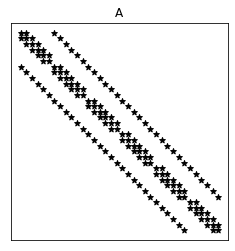
\includegraphics[width=0.45\textwidth]{cap_sislin/dados/figPoissonDnhIlu0/A}~
  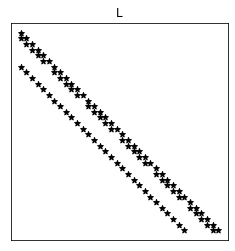
\includegraphics[width=0.45\textwidth]{cap_sislin/dados/figPoissonDnhIlu0/L}\\
  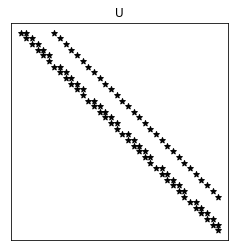
\includegraphics[width=0.45\textwidth]{cap_sislin/dados/figPoissonDnhIlu0/U}~
  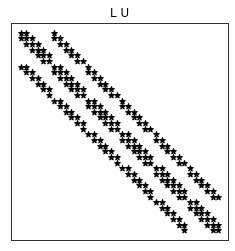
\includegraphics[width=0.45\textwidth]{cap_sislin/dados/figPoissonDnhIlu0/LU}
  \caption{Representação das matrizes ILU(0).}
  \label{fig:poissonDnhIlu0}
\end{figure}

\begin{ex}{ex:possoinDnhIlu0}
  Consideramos o sistema linear $Ax = b$ associado ao problema discreto trabalhado no Exercício \ref{exer:poissonDNH}. Para uma malha $n\times n=8\times 8$, obtemos as matrizes representadas na Figura \ref{fig:poissonDnhIlu0}.

  Observamos que a matriz $LU$ contém duas diagonais com elementos não nulos a mais que a matriz original $A$. Estes elementos são chamados de {\it fill-in}. 
\end{ex}


\lstinputlisting[caption=Algoritmo ILU(0), label={lst:algIlu0}]{./cap_sislin/dados/pyIlu0/main.py}

\subsubsection{Exercícios}
\badgeRevisar

\begin{exer}
  Considere o problema discreto do Exercício \ref{exer:poissonDNH}.
  \begin{enumerate}[a)]
  \item Compute a solução com o método GMRES com precondicionamento ILU(0).
  \item Compare com a resolução com o método GMRES sem precondicionamento.
  \item Compare com a resolução com o método CG sem precondicionamento.
  \item O precondicionamento ILU(0) é eficiente para o método CG?
  \end{enumerate}
\end{exer}

\chapter{Sistemas Não Lineares e Otimização}\label{cap_otimizacao}
\badgeRevisar

Neste capítulo, apresentam-se métodos numéricos para a resolução de sistemas não lineares e de problemas de otimização. Salvo explicitado ao contrário, assume-se que os problemas são bem definidos.

\section{Sistemas Não-Lineares}\label{cap_otimizacao_sec_sisnlin}
\badgeRevisar

Consideramos o seguinte problema: \hl{dada a função $F:D\subset \mathbb{R}^n\to\mathbb{R}^n$ encontrar $\pmb{x}^*\in\mathbb{R}^n$ tal que}
\begin{equation}\hleq
  F(\pmb{x}^*) = 0.
\end{equation}
Salvo explicitado ao contrário, assumiremos que $F\in C^1(D)$, i.e. $F$ é uma função continuamente diferenciável no domínio computacional $D\subset\mathbb{R}^n$. 

Vamos, denotar por $J_F(\pmb{x}) = [\jmath_{i,j}(\pmb{x})]_{i,j=1}^{n,n}$ a \hlemph{matriz jacobiana}{\jacobi} da F com
\begin{equation}\hleq
  \jmath_{i,j}(\pmb{x}) = \frac{\p f_i(\pmb{x})}{\p x_j},
\end{equation}
onde $F(\pmb{x}) = (f_1(\pmb{x}), f_2(\pmb{x}), \dotsc, f_n(\pmb{x}))$ e $\pmb{x} = (x_1, x_2,\dotsc, x_n)$.

\subsection{Método de Newton}\label{cap_otimizacao_sec_sisnlin_ssec_newton}
\badgeRevisar

A iteração básica do \hlemph{método de Newton}{\newton} para sistemas de equações consiste em: dada uma aproximação inicial $\pmb{x}^{(0)}\in\mathbb{R}^n$,
\begin{align}
  &\text{resolver}\quad \hleq J_F\left(\pmb{x}^{(k)}\right)\pmb{\delta}^{(k)} = -F\left(\pmb{x}^{(k)}\right)\\
  &\text{computar}\quad \hleq \pmb{x}^{(k+1)} = \pmb{x}^{(k)} + \pmb{\delta}^{(k)}
\end{align}
para $k = 0, 1, 2, \ldots$ até que um critério de parada seja satisfeito.

\begin{obs}[\hl{Convergência}]\label{cap_otimizacao_sec_newton:obs:convNewton}
  Para $\pmb{x}^{(0)}$ suficientemente próximo da solução $\pmb{x}^*$, \hl{o método de Newton é quadraticamente convergente}. Mais precisamente, este resultado de convergência local requer que $J_F^{-1}(\pmb{x}^*)$ seja não singular e que $J_F$ seja Lipschitz{\lipschitz} contínua. Consulte \cite[Seção 7.1]{Quarteroni2007a} para mais detalhes.
\end{obs}

\begin{ex}\label{cap_otimizacao_sec_sisnlin:ex:burgers}
  Consideramos a \emph{equação de Burgers}{\burgers}
  \begin{equation}
    \frac{\p u}{\p t} + u\frac{\p u}{\p x} = \nu\frac{\p^2 u}{\p x^2}
  \end{equation}
  com $\nu>0$, condição inicial
  \begin{equation}
    u(0,x) = -\sen(\pi x)
  \end{equation}
  e condições de contorno de Dirichlet{\dirichlet} homogêneas
  \begin{equation}
    u(t,-1) = u(t,1) = 0.
  \end{equation}

  Aplicando o \emph{método de Rothe}{\rothe} com aproximação de Euler{\euler} implícita, obtemos
  \begin{equation}
    \begin{aligned}
      & \frac{u(t+h_t,x) - u(t,x)}{h_t} +\\
      &\quad u(t+h_t,x)u_x(t+h_t,x) \approx \nu u_{xx}(t+h_t,x),
    \end{aligned}
  \end{equation}
  onde $h_t>0$ é o passo no tempo. Agora, aplicamos diferenças finitas para obter
  \begin{equation}
    \begin{aligned}
      &\frac{u(t+h_t,x_i) - u(t,x_i)}{h_t} \\
      &\quad + u(t+h_t, x_i)\frac{u(t+h_t,x_{i+1})-u(t+h_t,x_{i-1})}{2h_x} \\
      &\quad \approx \nu\frac{u(t+h_t,x_{i-1}) - 2u(t+h_t,x_i) + u(t+h_t,x_{i+1})}{h_x^2},
    \end{aligned} 
 \end{equation}
  onde, $x_i=(i-1)h_x$, $i=1,\dotsc,n_x$ e $h_x=1/(n_x-1)$ é o tamanho da malha.

  Rearranjando os termos e denotando $u^{(k)}_i\approx u(t_k, x_i)$, $t_k = (k-1)h$, obtemos o seguinte \emph{problema discreto}
  \begin{align}
    & u^{(k+1)}_1 = 0\\
    & \frac{1}{h_t}u^{(k+1)}_i - \frac{1}{h_t}u^{(k)}_i + \frac{1}{2h_x}u^{(k+1)}_iu^{(k+1)}_{i+1} \nonumber\\
    &\quad - \frac{1}{2h_x}u^{(k+1)}_{i}u^{(k+1)}_{i-1} - \frac{\nu}{h_x^2}u^{(k+1)}_{i-1} \nonumber\\ 
    &\quad + 2\frac{\nu}{h_x^2}u^{(k+1)}_i - \frac{\nu}{h_x^2}u^{(k+1)}_{i+1} = 0,\\
    & u^{(k+1)}_{n_x} = 0,
  \end{align}
  sendo $u^{(0)}_i = -\sen(\pi x_i)$, $i = 1, \dotsc, n_x$ e $k = 1, 2, \ldots$.

  Este problema pode ser reescrito como segue: para cada $k = 0, 1, \ldots$, encontrar $\pmb{w}\in\mathbb{R}^{n_x}$, tal que
  \begin{equation}
    F\left(\pmb{w}; \pmb{w}^{(0)}\right) = 0, 
  \end{equation}
  onde $w_{i} = u^{(k+1)}_i$, $w_{i}^{(0)} = u^{(k)}_{i}$ e
  \begin{align}
    & f_1\left(\pmb{w}; \pmb{w}^{(0)}\right) = w_1,\\
    & f_{i}\left(\pmb{w}; \pmb{w}^{(0)}\right) = \frac{1}{h_t}w_i - \frac{1}{h_t}w^{(0)}_i + \frac{1}{2h_x}w_iw_{i+1} \nonumber\\
    &\quad - \frac{1}{2h_x}w_iw_{i-1} - \frac{\nu}{h_x^2}w_{i-1} + 2\frac{\nu}{h_x^2}w_i - \frac{\nu}{h_x^2}w_{i+1},\\
    &f_{n_x}\left(\pmb{w}; \pmb{w}^{(0)}\right) = w_{n_x}.
  \end{align}
  A matriz jacobiana associada $J=[\jmath_{i,j}]_{i,j}^{n_x,n_x}$ contém
  \begin{align}
    & \jmath_{i,j} = 0,\quad j\neq i-1,i,i+1,\\
    & \jmath_{1,1} = 1,\\
    & \jmath_{1,2} = 0,\\
    & \jmath_{i,i-1} = \frac{1}{2h_x}w_i - \frac{\nu}{h_x^2},\\
    & \jmath_{i,i} = \frac{1}{h_t} + \frac{1}{2h_x}w_{i+1} - \frac{2}{h_x}w_{i-1} + \frac{2\nu}{h_x^2},\\
    & \jmath_{i,i+1} = \frac{1}{2h_x}w_{i} - \frac{\nu}{h_x^2},\\
    & \jmath_{n_x,n_x-1} = 0\\
    & \jmath_{n_x,n_x} = 1.
  \end{align}

  Implemente este esquema numérico!
\end{ex}

\begin{exer}\label{cap_otimizacao_sec_sisnlin:exer:burgers}
  Considere o problema discreto apresentado no Exemplo~\ref{cap_otimizacao_sec_sisnlin:ex:burgers} para diferentes valores do coeficiente de difusão $\nu = \nu_0/\pi$, $\nu_0 = 1., 0.1, 0.01, 0.001$. Simule o problema com cada uma das seguintes estratégias e as compare quanto ao desempenho computacional.
  \begin{enumerate}[a)]
  \item Simule-o aplicando o Método de Newton com o {\it solver} linear \lstinline+npla.solve+.
  \item Observe que a jacobiana é uma matriz tridiagonal. Simule o problema aplicando o Método de Newton com o {\it solver} linear \lstinline+npla.solve_banded+.
  \item Aloque a jacobiana como uma matriz esparsa. Então, simule o problema aplicando o Método de Newton com {\it solver} linear adequado para matrizes esparsas.
  \end{enumerate}
\end{exer}

\begin{exer}
  Desenvolva um esquema \textit{upwind} para simular a equação de Burgers do Exemplo~\ref{cap_otimizacao_sec_sisnlin:ex:burgers}.
\end{exer}

\subsection{Método Tipo Newton}\label{cap_otimizacao_sec_sisnlin_ssec_tipoNewton}
\badgeRevisar

Existem várias modificações do Método de Newton{\newton} que buscam reduzir o custo computacional. Há estratégias para simplificar as computações da matriz jacobiana{\jacobi} e para reduzir o custo nas computações das atualizações de Newton.

\subsubsection{Atualização Cíclica da Matriz Jacobiana}
\badgeRevisar

Geralmente, ao simplificarmos a matriz jacobina $J_F$ ou aproximarmos a atualização de Newton $\delta^{(k)}$, perdemos a convergência quadrática do método (consulte a Observação \ref{obs:convNewton}). A ideia é, então, buscar uma convergência pelo menos super-linear, i.e.
\begin{equation}
  \|e^{(k+1)}\|\approx \rho_k\|e^{(k)}\|,
\end{equation}
com $\rho_k\to 0$ quando $k\to\infty$. Aqui, $e^{(k)}:=x^*-x^{(k)}$. Se a convergência é superlinear, então podemos usar a seguinte aproximação
\begin{equation}
  \rho_k \approx \frac{\|\delta^{(k)}\|}{\|\delta^{(k-1)}\|}
\end{equation}
ou, equivalentemente,
\begin{equation}
  \rho_k \approx \left(\frac{\|\delta^{(k)}\|}{\|\delta^{(0)}\|}\right)^{\frac{1}{k}}
\end{equation}
Isso mostra que podemos acompanhar a convergência das iterações pelo fator
\begin{equation}
  \beta_k = \frac{\|\delta^{(k)}\|}{\|\delta^{(0)}\|}.
\end{equation}
Ao garantirmos $0<\beta_k<1$, deveremos ter uma convergência superlinear.

Vamos, então, propor o seguinte  método tipo Newton de atualização cíclica da matriz jacobiana.
\begin{enumerate}
\item Escolha $0<\beta<1$
\item $J := J_F(x^{(0)})$
\item $J\delta^{(0)}=-F(x^{(0)})$
\item $x^{(1)} = x^{(0)} + \delta^{(0)}$
\item Para $k=1,\ldots$ até critério de convergência:
  \begin{enumerate}
  \item $J\delta^{(k)}=-F(x^{(k)})$
  \item $x^{(k+1)}=x^{(k)} + \delta^{(k)}$
  \item Se $\|\delta^{(k)}\|/\|\delta^{(0)}\| > \beta$:
    \begin{enumerate}
    \item $J := J_F(x^{(k)})$
    \end{enumerate}
  \end{enumerate}
\end{enumerate}

\begin{exer}
  Implemente uma versão do Método Tipo Newton apresentado acima e aplique-o para simular o problema discutido no Exemplo \ref{ex:burgers} para $\nu = 1., 0.1, 0.01, 0.001, 0.0001$. Faça uma implementação com suporte para matrizes esparsas.
\end{exer}

\section{Problemas de Minimização}\label{cap_otimizacao_sec_minimi}
\badgeRevisar

Vamos considerar o seguinte \hl{\emph{problema de minimização}: dada a \emph{função objetivo} $f:D\subset \mathbb{R}^n\to\mathbb{R}$, resolver}
\begin{equation}\hleq
  \min_{\pmb{x}\in D} f(\pmb{x}).
\end{equation}
No que segue e salvo dito explicitamente ao contrário, vamos assumir que o problema está bem determinado e que $f$ é suficientemente suave. Ainda, vamos assumir as seguintes notações:
\begin{itemize}
\item gradiente de $f$
  \begin{equation}
    \nabla f(\pmb{x}) = \left(\frac{\p f}{\p x_1}(\pmb{x}),\dotsc,\frac{\p f}{\p x_n}(\pmb{x})\right)
  \end{equation}
\item derivada direcional de $f$ com respeito a $\pmb{d}\in\mathbb{R}^n$
  \begin{equation}
    \frac{\p f}{\p \pmb{d}}(\pmb{x}) = \nabla f(\pmb{x})\cdot \pmb{d}
  \end{equation}
\item matriz hessiana de $f$, $H=[h_{i,j}]_{i,j=1}^{n,n}$
  \begin{equation}
    h_{i,j}(\pmb{x}) = \frac{\p^2 f}{\p x_i\p x_j}(\pmb{x})
  \end{equation}
\end{itemize}

\begin{obs}[\hl{Condições de Otimização}]
  Se $\nabla f(\pmb{x}^*) = 0$ e $H(\pmb{x}^*)$ é positiva definida, então $\pmb{x}^*$ é um mínimo local de $f$ em uma vizinhança não vazia de $\pmb{x}^*$. Consulte mais em \cite[Seção 7.2]{Quarteroni2007a}. Um ponto $\pmb{x}^*$ tal que $\nabla f(\pmb{x}^*) = 0$ é chamado de \hlemph{ponto crítico}.
\end{obs}

\subsection{Métodos de Declive}
\badgeRevisar

Um \hl{\emph{método de declive} consiste em uma iteração tal que: dada uma aproximação inicial $\pmb{x}^{(0)}\in\mathbb{R}^n$, computa-se}
\begin{equation}\hleq
  \pmb{x}^{(k+1)} = \pmb{x}^{(k)} + \alpha^{(k)} \pmb{d}^{(k)},
\end{equation}
com \hlemph{tamanho de passo} $\alpha^{(k)}>0$, para $k=0,1,2,\ldots$ até que um dado critério de parada seja satisfeito. As \hlemph{direções descendentes} são tais que
\begin{align}
  &\hleq \pmb{d}^{(k)}\cdot\nabla f(\pmb{x}^{(k)}) < 0,\quad \text{se } \nabla f(\pmb{x}^{(k)}) \neq 0,\label{eq:condDirecoes0}\\
  &\hleq \pmb{d}^{(k)} = 0,\quad \text{noutro caso.}\label{eq:condDirecoes1}
\end{align}

\begin{obs}[\hl{Condição de Convergência}]
  Da Série de Taylor{\taylor}, temos que
  \begin{equation}
    f(\pmb{x}^{(k)}+\alpha^{(k)}\pmb{d}^{(k)}) - f(\pmb{x}^{(k)}) = \alpha^{(k)}\nabla f(\pmb{x}^{(k)})\cdot \pmb{d}^{(k)} + \varepsilon,
  \end{equation}
  com $\varepsilon\to 0$ quando $\alpha^{(k)}\to 0$. Como consequência da continuidade da $f$, para $\alpha^{(k)}$ suficientemente pequeno, o sinal do lado esquerdo é igual a do direito desta última equação. Logo, para tais $\alpha^{(k)}$ e $\pmb{d}^{(k)}\neq 0$ uma direção descendente, temos garantido que
  \begin{equation}
    f(\pmb{x}^{(k)}+\alpha^{(k)}\pmb{d}^{(k)}) < f(\pmb{x}^{(k)}).
  \end{equation}
\end{obs}


\hl{Notamos que um método de declive fica determinado pelas escolhas da direção de declive $\pmb{d}^{(k)}$ e o tamanho do passo $\alpha^{(k)}$}. Primeiramente, vamos a este último item.

\subsubsection{Pesquisa linear}
\badgeRevisar

O \hl{\emph{método de pesquisa linear} consiste em escolher $\alpha^{(k)}$ com base na resolução do seguinte problema de minimização}
\begin{equation}\hleq
  \min_{\alpha\in\mathbb{R}} \phi(\alpha) := f(\pmb{x}^{(k)}+\alpha \pmb{d}^{(k)}).
\end{equation}
Entretanto, a resolução exata deste problema é muitas vezes não factível. \hl{Técnicas de aproximações para a resolução deste problema são}, então, aplicadas. Tais técnicas são \hl{chamadas de \emph{pesquisa linear não exata}}.

A \hl{\emph{condição de Armijo} é que a escolha de $\alpha^{(k)}$ deve ser tal que}
\begin{equation} \label{eq:condArmijo}\hleq
  f\left(\pmb{x}^{(k)}+\alpha^{(k)} \pmb{d}^{(k)}\right) \leq f(\pmb{x}^{(k)}) + \sigma \alpha^{(k)} \nabla f\left(\pmb{x}^{(k)}\right)\cdot \pmb{d}^{(k)},
\end{equation}
\hl{para alguma constante $\sigma\in (0, 1/2)$}. Ou seja, a redução em $f$ é esperada ser proporcional à derivada direcional de $f$ com relação a direção $\pmb{d}^{(k)}$ no ponto $\pmb{x}^{(k)}$. Em aplicações computacionais, $\sigma$ é normalmente escolhido no intervalo $[10^{-5}, 10^{-1}]$.

A condição \eqref{eq:condArmijo} não é suficiente \hl{para evitar escolhas muito pequenas de $\alpha^{(k)}$}. Para tanto, \hl{pode-se empregar a \emph{condição de curvatura}}, a qual requer que
\begin{equation}\label{eq:condCurvatura}\hleq
  \nabla f\left(\pmb{x}^{(k)} + \alpha^{(k)}\pmb{d}^{(k)}\right)\cdot \pmb{d}^{(k)} \geq \beta\nabla f\left(\pmb{x}^{(k)}\right)\cdot\pmb{d}^{(k)},
\end{equation}
\hl{para $\beta\in [\sigma, 1/2]$}. Notemos que o lado esquerdo de \eqref{eq:condCurvatura} é igual a $\phi'(\alpha^{(k)})$. Ou seja, este condição impõe que $\alpha^{(k)}$ seja maior que $\beta\phi'(0)$. Normalmente, escolhe-se $\beta\in [10^{-1}, 1/2]$. \hl{Juntas}, \eqref{eq:condArmijo} e \eqref{eq:condCurvatura} \hl{são conhecidas como \emph{condições de Wolfe}}{\wolfe}.

\subsection{Método do Gradiente}
\badgeRevisar

\hl{O \emph{método do gradiente} (ou método do máximo declive) é um método de declive tal que as direções descendentes são o oposto do gradiente da $f$, i.e.}
\begin{equation}
  \pmb{d}^{(k)} = -\nabla f(\pmb{x}^{(k)}).
\end{equation}
É imediato verificar que as condições \eqref{eq:condDirecoes0}-\eqref{eq:condDirecoes1} são satisfeitas.

\begin{ex}\label{ex:Rosenbrock}
  Consideramos o problema de encontrar o mínimo da \emph{função de Rosenbrock}{\rosenbrock}
  \begin{equation}
    f(\pmb{x}) = \sum_{i=1}^n 100\left(x_{i+1}-x_i^2\right)^2 + (1-x_i)^2.
  \end{equation}
  O valor mínimo desta função é zero e ocorre no ponto $\pmb{x} = \pmb{1}$. Esta função é comumente usada como caso padrão para teste de métodos de otimização.

  Para o método do gradiente, precisamos das derivadas parciais
  \begin{align}
    & \frac{\p f}{\p x_1} = -400x_1\left(x_2-x_1^2\right) - 2(1-x_1) \\
    &  \frac{\p f}{\p x_j} = \sum_{i=1}^n 200\left(x_i-x_{i-1}^2\right)(\delta_{i,j} - 2x_{i-1}\delta_{i-1,j}) \nonumber\\
    &\qquad - 2(1-x_{i-1})\delta_{i-1,j} \\
    & \frac{\p f}{\p x_{n}} = 200\left(x_n - x_{n-1}^2\right)
  \end{align}
  onde, $\delta_{i,j}$ é o delta de Kronecker{\kronecker}.


\begin{lstlisting}[caption=Algoritmo do Gradiente, label={lst:algOtimMG}]
import numpy as np
import numpy.linalg as npla
import scipy.optimize as spopt

# fun obj
def fun(x):
  '''
  Função de Rosenbrock
  '''
  return sum(100.*(x[1:]-x[:-1]**2.)**2. + (1.-x[:-1])**2.)

# gradiente da fun
def grad(x):
  xm = x[1:-1]
  xm_m1 = x[:-2]
  xm_p1 = x[2:]
  der = np.zeros_like(x)
  der[1:-1] = 200*(xm-xm_m1**2) - 400*(xm_p1 - xm**2)*xm - 2*(1-xm)
  der[0] = -400*x[0]*(x[1]-x[0]**2) - 2*(1-x[0])
  der[-1] = 200*(x[-1]-x[-2]**2)
  
  return der

# problem dimension
n = 2

# num max iters
maxiter = 100000
# tolerancia
tol = 1e-10

# aprox. inicial
x = np.zeros(n)

for k in range(maxiter):
  # direcao descendente
  d = -grad(x)

  # pesquisa linear
  alpha = spopt.line_search(fun, grad, x, d, 
                            c1=0.0001, c2=0.9)[0]

  # atualizacao
  x = x + alpha * d

  nad = npla.norm(alpha * d)
  nfun = npla.norm(fun(x))

  if ((k+1) % 10 == 0):
    print(f"{k+1}: {alpha:1.2e} {nad:1.2e} {nfun:1.2e}")

  if (nfun < tol):
    break
\end{lstlisting}

\end{ex}

\subsubsection{Exercícios}
\badgeRevisar

\begin{exer}
  Aplique o método do gradiente para computar o ponto mínimo da função de Rosenbrock{\rosenbrock}
  \begin{equation}
    f(\pmb{x}) = \sum_{i=1}^n 100\left(x_{i+1}-x_i^2\right)^2 + (1-x_i)^2
  \end{equation}
  com
  \begin{enumerate}
    \item $n = 2$.
    \item $n = 3$.
    \item $n = 4$.
    \item $n = 5$.
    \item $n = 10$.
  \end{enumerate}
\end{exer}
\begin{resp}
$f(\pmb{1}) = 0$
\end{resp}

\begin{exer}
  Aplique o método do gradiente para computar o ponto mínimo da função de Beale \cite{Beale1955a}
  \begin{equation}
    \begin{aligned}
      & f(x,y) = (1.5-x+xy)^2 \\
      &\qquad + (2.25-x+xy^2)^2 \\
      &\qquad + (2.625-x+xy^3)^2.
    \end{aligned}
  \end{equation}
  para $\pmb{x}\in [-4.5, 4.5]^2$.
\end{exer}
\begin{resp}
  $f(3, 0.5) = 0$
\end{resp}

\begin{exer}
  Aplique o método do gradiente para computar o ponto mínimo da função de Goldstein-Price \cite{Goldstein1971a}
  \begin{equation}
    \begin{aligned}
      & f(x,y) = \left[1+\left(x+y+1\right)^{2}\left(19-14x \right.\right.\\
      &\qquad \left.\left.+ 3x^{2}-14y+6xy+3y^{2}\right)\right] \\
      &\qquad \times \left[30+\left(2x-3y\right)^{2}\left(18-32x\right.\right.\\
      &\qquad \left.\left.+12x^{2}+48y-36xy+27y^{2}\right)\right]
    \end{aligned}  
  \end{equation}
\end{exer}
\begin{resp}
  $f(0,-1) = 3$
\end{resp}

\begin{exer}
  Aplique o método do gradiente para computar o ponto mínimo da função de Booth
  \begin{equation}
    f(x,y) = \left( x + 2y -7\right)^{2} + \left(2x +y - 5\right)^{2}
  \end{equation}
  para $\pmb{x}\in [-10, 10]^2$.
\end{exer}
\begin{resp}
  $f(1,3)=0$
\end{resp}

\begin{exer}
  Aplique o método do gradiente para computar o ponto mínimo da função de Rastrigin
  \begin{equation}
    f(x) = 10 n + \sum_{i=1}^n \left[x_i^2 - 10\cos(2 \pi x_i)\right],
  \end{equation}
  para $\pmb{x}\in[-5.12, 5.12]^n$, com
  \begin{enumerate}
    \item $n = 2$.
    \item $n = 3$.
    \item $n = 4$.
    \item $n = 5$.
    \item $n = 10$.
  \end{enumerate}
\end{exer}
\begin{resp}
$f(\pmb{0}) = 0$
\end{resp}


\subsection{Método de Newton}
\badgeRevisar

O Método de Newton{\newton} para problemas de otimização é um Método de Declive com direções descendentes
\begin{equation}
  d^{(k)} = -H^{-1}(x^{(k)})\nabla f(x^{(k)}),
\end{equation}
assumindo que a hessiana $H$ seja definida positiva dentro de uma vizinhança suficientemente grande do ponto de mínimo $x^*$.

\begin{obs}
  A cada iteração de Newton é necessário computar a inversa da matriz hessiana. Este é um passo crítico para o desempenho computacional. Desta forma, a escolha do método para o cálculo da inversa é normalmente explicitado, este é chamado de {\it solver} linear. Por exemplo, \emph{Newton-Krylov} é o nome dado ao Método de Newton que utiliza um Método de Subespaço de Krylov como {\it solver} linear. Mais especificamente, \emph{Newton-GMRES} quando a inversa é computada com o GMRES. Uma escolha natural é \emph{Newton-GC}, tendo em vista que o Método de Gradiente Conjugado é ideal para matriz simétrica e definida positiva.
\end{obs}

\begin{obs}
  Na implementação computacional não é necessário computar a inversa da hessiana, mais apenas computar $d^{(k)}$ resolvendo o seguinte sistema linear
  \begin{equation}
    H(x^{(k)})d^{(k)} = -\nabla f(x^{(k)}).
  \end{equation}
\end{obs}

\begin{ex}\label{ex:optNewtonGC}
  Seguindo o Exemplo \ref{ex:Rosenbrock}, temos que a hessiana associada é a matriz simétrica $H = [h_{i,j}]_{i,j=1}^{n,n}$ com
  \begin{align}
    h_{1,1} &= \frac{\p^2 f}{\p x_1^2} = 1200x_1^2-400x_2+2\\
    h_{1,2} &= \frac{\p^2 f}{\p x_1\p x_2} = -400x_1\\
            &~\nonumber\\
    h_{i,j} &= \frac{\p^2 f}{\p x_i\p x_j} = 200(\delta_{i,j}-2x_{i-1}\delta_{i-1,j}) - 400(\delta_{i+1,j}-2x_i\delta_{i,j})\nonumber\\
            &- 400\delta_{i,j}(x_{i+1}-x_i^2) + 2\delta_{i,j}\\
            &~\nonumber\\
    h_{n-1,n} &= \frac{\p^2 f}{\p x_{n-1}\p x_n} = -400x_{n-1}\\
    h_{n,n} &= \frac{\p^2 f}{\p x_{n-1}} = 200
  \end{align}
  Notemos que a hessiana é uma matriz tridiagonal.

  \lstinputlisting[caption=Algoritmo de Newton, label={lst:algOtimNewton}]{./cap_otimizacao/dados/pyNewton/main.py}  
\end{ex}

\begin{obs}{Métodos Tipo Newton}
  Métodos Tipo Newton são aqueles que utilizam uma aproximação para a inversa da matriz hessiana. Uma estratégia comumente aplicada, é a de atualizar a hessiana apenas em algumas iterações, baseando-se em uma estimativa da taxa de convergência. Na Seção \ref{cap_otimizacao_sec_tipoNewton}, exploramos esta técnica no contexto de resolução de sistemas não lineares.
\end{obs}

\begin{exer}
  Aplique o Método de Newton para minimizar a função de Rosenbrock no caso de várias dimensões. Para tanto, utilize uma implementação eficiente com suporte para matrizes esparsas. Compare o desempenho entre os métodos Newton-GMRES e Newton-GC. 
\end{exer}

\begin{exer}
  Aplique o Método de Newton para minimizar as funções dadas no Exercício \ref{exer:optFuns}.
\end{exer}

\subsection{Método do Gradiente Conjugado}
\badgeRevisar

Métodos do Gradiente Conjugado são obtidos escolhendo-se as direções descendentes
\begin{equation}
  d^{(k)} = -\nabla f(x^{(k)}) + \beta_k d^{(k-1)},
\end{equation}
onde $\beta_k$ é um escalar escolhido de forma que as direções $\{d^{(k)}\}$ sejam mutuamente ortogonais com respeito a uma dada norma. Por exemplo, o \emph{Método de Fletcher}-\emph{Reeves} consiste em escolher
\begin{equation}
  \beta_k = \frac{\nabla f(x^{(k)})\cdot\nabla f(x^{(k)})}{\nabla f(x^{(k-1)})\cdot\nabla f(x^{(k-1)})},
\end{equation}
o que garante que as direções sejam mutuamente ortogonais com respeito ao produto interno euclidiano.

\begin{obs}
  Outras variações comumente empregadas são o Método de Polak-Ribière e suas variantes. Consulte mais em \cite[Seção 5.2]{Nocedal2006}.
\end{obs}

\begin{ex}
  Implementação do Método de Fletcher-Reeves para a minimização da função de Rosenbrock dada no Exemplo \ref{ex:Rosenbrock}.
  
  \lstinputlisting[caption=Algoritmo de Fletcher-Reeves, label={lst:algOtimGC}]{./cap_otimizacao/dados/pyMGC/main.py}    
\end{ex}

\begin{exer}
  Teste o Método de Fletcher-Reeves para a minimização das funções dadas no Exercício \ref{exer:optFuns}.
\end{exer}
\chapter{Autovalores e Autovetores}\label{cap_autoval}
\badgeRevisar

Neste capítulo, estudamos métodos numéricos para a computação de autovalores e autovetores de matrizes.

\section{Método da Potência}\label{cap_autoval_sec_pot}
\badgeRevisar

\hl{O \emph{método da potência} é uma técnica iterativa para computar o autovalor dominante de uma matriz e um autovetor associado}. Modificações do método, tornam possível sua aplicação para a determinação de outros autovalores próximos a um número dado. Desta forma, pode ser utilizá-lo em conjunto com outra técnica de aproximação de autovalores e autovetores.

\subsection{Autovalor dominante}
\badgeRevisar

Vamos denotar o \emph{espectro} de uma dada matriz $A\in\mathbb{C}^{n\times n}$ por
\begin{equation}
  \sigma(A) = \{\lambda_1, \lambda_2, \dotsc, \lambda_n\},
\end{equation}
sendo $\lambda_i\in \mathbb{C}$ o $i$-ésimo \emph{autovalor} de uma \emph{matriz diagonalizável}\endnote{Existe uma base de $\mathbb{C}^{n\times n}$ formada apenas de autovetores de $A$.} $A=[a_{i,j}]_{i,j=1}^{n,n}$, i.e. existe um vetor $\pmb{0}\neq \pmb{v}_i\in\mathbb{C}^n$ tal que
\begin{equation}\hleq
  A\pmb{v}_i = \lambda_i \pmb{v}_i,
\end{equation}
sendo $\pmb{v}_i$ chamado de \emph{autovetor} associado a $\lambda_i$. No desenvolvimento do \emph{método da potência}, vamos assumir que os autovalores podem ser ordenados da seguinte forma
\begin{equation}\hleq
  |\lambda_1| > |\lambda_2| \geq \cdots \geq |\lambda_n|.
\end{equation}
Assim sendo, o \hl{$\lambda_1$ é chamado de \emph{autovalor dominante}}. Na sequência, vamos denotar por $\pmb{A}^H$ a transposta conjugada de $A$, i.e. $A^H=[\bar{a}_{j,i}]_{i,j=1}^{n,n}$.

\hl{A \emph{iteração} do método da potência consiste em}
\begin{align}\hleq
  & \pmb{z}^{(k)} = A\pmb{q}^{(k-1)},\\
  & \pmb{q}^{(k)} = \pmb{z}^{(k)}/\left\|\pmb{z}^{(k)}\right\|,\\
  & \nu^{(k)} = (\pmb{q}^{(k)})^H A \pmb{q}^{(k)},
\end{align}
com dada aproximação inicial $\pmb{q}^{(0)}$ para um autovetor associado a $\lambda_1$. Quando o método é bem sucedido, tem-se $\nu^{(k)}\to \lambda_1$ quando $k\to\infty$.

\subsubsection{Convergência}

Para mostrar a convergência do método, basta mostrar que $\pmb{q}^{(k)}$ converge para um autovetor associado a $\lambda_1$. Primeiramente, notamos que\endnote{Segue por indução matemática.}
\begin{equation}
  \pmb{q}^{(k)} = \frac{A^k\pmb{q}^{(0)}}{\left\|A^k\pmb{q}^{(0)}\right\|}, ~k\geq 1.
\end{equation}
Para $A$ diagonalizável, temos que existe uma base $\left\{\pmb{v}_1, \pmb{v}_2, \dotsc, \pmb{v}_n\right\}$ de $\mathbb{C}^{n\times n}$ formada apenas de autovetores de $A$. Segue que
\begin{equation}\label{eq:q0_comblin}
  \pmb{q}^{(0)} = \sum_{i=1}^n \alpha_i \pmb{v}_i,
\end{equation}
onde $\alpha_i\in\mathbb{C}$. Vamos assumir que $\alpha_1\neq 0$\endnote{Condição necessária para a convergência.}. Ainda, $A\pmb{v}_i = \lambda_i \pmb{v}_i$, donde
\begin{align}
  A^k\pmb{q}^{(0)} &= \sum_{i=1}^n \alpha_iA^k\pmb{v}_i\\
             &= \sum_{i=1}^n \alpha_i\lambda_i^k\pmb{v}_i\\
             &= \alpha_1\lambda_1^k\left[\pmb{v}_1 + \sum_{i=2}^n\frac{\alpha_i}{\alpha_1}\left(\frac{\lambda_k}{\lambda_1}\right)^k\pmb{v}_i\right]
\end{align}
Como $|\lambda_i|/|\lambda_1| < 1$, $i=2,\dotsc,n$, temos que
\begin{equation}
  \pmb{y}^{(k)} = \sum_{i=2}^n\frac{\alpha_i}{\alpha_1}\left(\frac{\lambda_k}{\lambda_1}\right)^k\pmb{v}_i \to 0,
\end{equation}
quando $k\to \infty$. Logo, temos que
\begin{align}
  \pmb{q}^{(k)} &= \frac{\alpha_1\lambda_1^k\left(\pmb{v}_1+\pmb{y}^{(k)}\right)}{\left\|\alpha_1\lambda_1\left(\pmb{v}_1+\pmb{y}^{(k)}\right)\right\|}\\
          &= \frac{\lambda_1}{|\lambda_1|}\frac{\left(\pmb{v}_1+\pmb{y}^{(k)}\right)}{\left\|\pmb{v}_1+\pmb{y}^{(k)}\right\|}.
\end{align}
Por fim, observamos que $\lambda_1/|\lambda_1|$ tem o mesmo sinal de $\lambda_1$. Portanto, $\pmb{q}^{(k)}$ tende a um múltiplo não nulo de $\pmb{v}_1$ quando $k\to\infty$.

\begin{observacao}[\hl{Aproximação Inicial}]
  A convergência do método da potência está condicionada a escolha de uma aproximação inicial tal que \eqref{eq:q0_comblin} seja tal que $\alpha_1\neq 0$. Não há como saber \textit{a priori} que o $\pmb{q}^{(0)}$ escolhido satisfaz essa condição e, caso não satisfaça as iterações não são convergentes.
\end{observacao}

\begin{obs}[\hl{Taxa de convergência}]
  Pode-se mostrar a seguinte taxa de convergência para o método da potência
  \begin{equation}
    \left\|\tilde{\pmb{q}}^{(k)}-\pmb{v}_1\right\| \leq C\left|\frac{\lambda_2}{\lambda_1}\right|^k,\quad k\geq 1,
  \end{equation}
  onde
  \begin{equation}
    \tilde{\pmb{q}}^{(k)} = \pmb{v}_1 + \sum_{i=2}^n \frac{\alpha_i}{\alpha_1}\left(\frac{\lambda_i}{\lambda_1}\right)^k\pmb{v}_i.
  \end{equation}
  Consulte \cite[Seção 5.3.]{Quarteroni2007a}.
\end{obs}

% \lstinputlisting[caption=Algoritmo do Método da Potência, label={lst:algMetPot}]{./cap_autoval/dados/pyMetPot/main.py}
\begin{lstlisting}[caption=Algoritmo do Método da Potência, label={lst:algMetPot}]
import numpy as np
import numpy.linalg as npla

def metPot(A, q0, maxiter=1000, tol=1e-14):
  q = q0/npla.norm(q0)
  nu0 = np.dot(q, A @ q)
  print(f"{0}: {nu0}")

  info = -1
  for k in range(maxiter):
    z = A @ q
    q = z/npla.norm(z)
    nu = np.dot(q, A @ q)

    print(f"{k+1}: {nu}")
    if (np.fabs(nu-nu0) < tol):
      info = 0
      break

    nu0 = nu

  return nu, q, info  
\end{lstlisting}

\subsubsection{Exercícios}

\begin{exer}
  Use o método da potência para computar o autovalor dominante da matriz de coeficientes do problema discreto associado ao Exercício~\ref{exer:pvc1d}. Estude sua convergência para diferentes tamanhos da matriz.
\end{exer}

\begin{exer}
  Use o método da potência para computar o autovalor dominante da matriz de coeficientes do problema discreto associado ao Exemplo~\ref{ex:poisson}. Estude sua convergência para diferentes tamanhos da matriz.
\end{exer}

\subsection{Método da Potência Inversa}
\badgeRevisar

Esta \hl{variação do método da potência nos permite computar o autovalor mais próximo de um número $\mu\in\mathbb{C}$ dado}, $\mu\not\in\sigma(A)$. A ideia é aplicar o método para a matriz
\begin{equation}
  M_\mu^{-1} = (A-\mu I)^{-1}.
\end{equation}
Neste contexto, \hl{$\mu$ é chamado de \emph{deslocamento}} (em inglês, {\it shift}).

Notamos que se $\left(\lambda_i, \pmb{v}_i\right)$ é um autopar de $A$, então $\xi_i=(\lambda_i-\mu)^{-1}$ é autovalor de $M_\mu^{-1}$ associado ao autovetor $\pmb{v}_i$. De fato,
\begin{align}
  & (\lambda_i - \mu) \pmb{v}_i = (A-\mu I)\pmb{v}_i \\
  & M_\mu^{-1}(\lambda_i-\mu)\pmb{v}_i = \pmb{v}_i \\
  & M_\mu^{-1}\pmb{v}_i = (\lambda_i-\mu)^{-1} \pmb{v}_i.
\end{align}
Isso também mostra que $A$ e $M_\mu^{-1}$ têm os mesmos autovetores.

Agora, \hl{se $\mu$ for suficientemente próximo de $\lambda_m$, autovalor simples de $A$, então}
\begin{equation}
  |\lambda_m-\mu| < |\lambda_i-\mu|,\quad i=1,2,\dotsc,n,~i\neq m.
\end{equation}
Com isso, \hl{$\xi_m=(\lambda_m-\mu)^{-1}$ é o autovalor dominante de $M_\mu^{-1}$} e, portanto, a iteração do método da potência aplicada a $M_\mu^{-1}$ fornece este autovalor. Mais especificamente, como $A$ e $M_\mu^{-1}$ tem os  mesmos autovetores, \hl{a \emph{iteração do método da potência inversa} é dada como segue}
\begin{align}
  & (A-\mu I)\pmb{z}^{(k)} = \pmb{q}^{(k-1)}, \label{eq:slmpi} \\
  & \pmb{q}^{(k)} = \pmb{z}^{(k)}/\|\pmb{z}^{(k)}\|, \\
  & \nu^{(k)} = (\pmb{q}^{(k)})^H A \pmb{q}^{(k)},
\end{align}
onde $\pmb{q}^{(0)}$ é uma aproximação inicial para o autovetor associado ao autovalor $\lambda_m$, $\nu^{(k)}\to \lambda_m$ quando $k\to \infty$.

\subsubsection{Exercícios}

\begin{exer}
  Use o método da potência para computar diferentes autovalores da matriz de coeficientes do problema discreto associado ao Exercício~\ref{exer:pvc1d}. Estude sua convergência para diferentes tamanhos da matriz. 
\end{exer}

\begin{exer}
  Use o método da potência para computar diferentes autovalores da matriz de coeficientes do problema discreto associado ao Exemplo~\ref{ex:poisson}. Verifique se há vantagem em aplicar os métodos GMRES e GC na resolução de \eqref{eq:slmpi}.
\end{exer}

\subsection{Métodos de Deflação}
\badgeConstrucao

%%% section
\section{Iteração QR}\label{cap_autoval_sec_qr}
\badgeRevisar

\hl{A \emph{iteração QR} é um método para a computação aproximada de todos os autovalores de uma dada matriz $A$}. A ideia é explorar um método iterativo para a computação da \emph{decomposição de Schur}{\schur} de A, i.e. encontrar uma \emph{matriz unitária}\endnote{Uma matriz $U$ é dita unitária quando $U^{-1} = U^H$.} $U$ tal que
\begin{equation}
  U^{H}AU =
  \begin{bmatrix}
    \lambda_1 & t_{12} & \cdots & t_{1n}\\
    0 & \lambda_2 & & t_{2n}\\
    \vdots & & \ddots & \vdots\\
    0 & \vdots & 0 & \lambda_n
  \end{bmatrix}
\end{equation}

Assumindo $A\in\mathbb{R}^{n\times n}$, sejam $Q^{(0)}\in\mathbb{R}^{n\times n}$ uma \emph{matriz ortogonal}\endnote{Uma matriz $Q$ é dita ortogonal quando $Q^TQ = I$.} e $T^{(0)} = (Q^{(0)})^TAQ^{(0)}$. A iteração $QR$ consiste em
\begin{align}
  &\text{determinar }Q^{(k)}, R^{(k)}\text{ tal que}\nonumber\\
  &Q^{(k)}R^{(k)} = T^{(k-1)} ~\text{(fatoração QR)}\\
  &T^{(k)} = R^{(k)}Q^{(k)},
\end{align}
para $k=1,2,\ldots$.

Ou seja, a cada iteração $k$, computa-se a fatoração da matriz $T^{(k-1)}$ como o produto de uma matriz ortogonal $Q^{(k)}$ com uma matriz triangular superior $R^{(k)}$. Então, computa-se uma nova aproximação $T^{(k)}$ pela multiplicação de $R^{(k)}$ por $Q^{(k)}$. Com isso, temos
\begin{align}
  & T^{(k)} = R^{(k)}Q^{(k)}\\
  &\text{}\quad = (Q^{(k)})^T(Q^{(k)}R^{(k)})Q^{(k)}\\
  &\text{}\quad = (Q^{(k)})^TT^{(k-1)}Q^{(k)}\\
  &\text{}\quad = (Q^{(k)})^TR^{(k-1)}Q^{(k-1)}Q^{(k)}\\
  &\text{}\quad = (Q^{(k)})^T(Q^{(k-1)})^TQ^{(k-1)}R^{(k-1)}Q^{(k-1)}Q^{(k)}\\
  &\text{}\quad = (Q^{(k-1)}Q^{(k)})^TT^{(k-2)}(Q^{(k-1)}Q^{(k)})\\
  &\text{}\quad =(Q^{(0)}\cdots Q^{(k)})^TA(Q^{(0)}\cdots Q^{(k)}).
\end{align}
Ou seja, $T^{(k)}$ é matriz semelhante a $A$ para todo $k$. E, portanto, tem os mesmos autovalres.

\begin{obs}[\hl{Convergência}]
  Se $A\in\mathbb{R}^{n\times n}$ for uma matriz com autovalores tais que
  \begin{equation}
    |\lambda_1| > |\lambda_2| > \cdots > |\lambda_n|,
  \end{equation}
  então
  \begin{equation}
    \lim_{k\to\infty} T^{(k)} =   \begin{bmatrix}
    \lambda_1 & t_{12} & \cdots & t_{1n}\\
    0 & \lambda_2 & & t_{2n}\\
    \vdots & & \ddots & \vdots\\
    0 & \vdots & 0 & \lambda_n
  \end{bmatrix}.
\end{equation}

  Para a taxa de convergência, temos
  \begin{equation}
    |t^{(k)}_{i,i-1}| = \mathcal{O}\left(\left|\frac{\lambda_i}{\lambda_{i-1}}\right|^k\right),\quad i=2,\dotsc,n,
  \end{equation}
  quando $k\to\infty$.

  Ainda, se $A$ for uma \emph{matriz simétrica}, então $T^{(k)}$ tende a uma matriz diagonal quando $k\to\infty$.
\end{obs}

\begin{obs}
  Variantes do método QR permitem sua aplicação para matrizes mais gerais. Consulte \cite{Golub2013a}.
\end{obs}

Uma forma eficiente do método QR é chamada de \emph{iteração Hessenberg}{\hessenberg}\emph{-QR}. Consiste em inicializar $T^{(0)}$ como uma \emph{matriz de Hessenberg superior}, i.e. $t^{(0)}_{i,j}=0$ para $i>j+1$. A computação de $T^{(0)}$ é feita com \emph{transformadas de Householder} e a fatoração $QR$ de $T^{(k)}$ utiliza de \emph{matrizes de Givens}{\givens}.

% \lstinputlisting[caption=Algoritmo da Iteração QR, label={lst:pyQRIter}]{./cap_autoval/dados/pyQRIter/main.py}
\begin{lstlisting}[caption=Algoritmo da Iteração QR, label={lst:pyQRIter}]
import numpy as np
import numpy.linalg as npla

def qr_iter(A, Q=None, maxiter=10, tol=1e-5):
  Q = np.eye(A.shape[0]) if Q==None else Q
  T0 = Q.T @ A @ Q
  info = -1
  for k in range(maxiter):
    Q, R = npla.qr(T0)
    T = R @ Q
    if (npla.norm(T-T0) < tol):
      info = 0
      break
    T0 = T
  return T, info  
\end{lstlisting}

\begin{obs}[\hl{Computação dos Autovetores}]
  Se $\pmb{v}$ é autovetor associado ao autovalor simples $\lambda$ de $A$, então
  \begin{align}
    & A\pmb{v} = \lambda \pmb{v}\\
    & (Q^{(k)})^TAQ^{(k)}(Q^{(k)})^T\pmb{v} \approx \lambda (Q^{(k)})^T\pmb{v}
  \end{align}
  Denotando, $y = (Q^{(k)})^T\pmb{v}$, temos
  \begin{equation}
    T^{(k)}\pmb{y} = \lambda \pmb{y}.
  \end{equation}

  Com isso, podemos computar $\pmb{y}$ e, então, temos $\pmb{v}\approx Q^{(k)}\pmb{y}$.
\end{obs}

\subsubsection{Exercícios}

\begin{exer}
  Use a iteração QR para computar os autovalores da matriz de coeficientes do problema discreto associado ao Exercício \ref{exer:pvc1d}.
\end{exer}

\begin{exer}
  Use a iteração QR para computar os autovalores da matriz de coeficientes do problema discreto associado ao Exemplo \ref{ex:poisson}. Use \lstinline+spla.hessenberg+ para computar $T^{(0)}$.
\end{exer}



\chapter{Integração}\label{cap_integracao}\index{integração}
\thispagestyle{fancy}

\section{Integral de Riemann}\label{cap_integracao_sec_riemann}\index{integral de!Riemann}

\begin{defn}\normalfont{(Partição de um intervalo)}\index{partição}
  Uma \emph{partição} $P$ de um intervalo $[a, b]$ é um conjunto ordenado da forma
  \begin{equation}
    P([a, b]) = \{a=x_0 < x_1 < x_2 < \ldots < x_n=b\}.
  \end{equation}
O valor $|P| = \max_{1\leq i\leq n} \Delta x_i$, $\Delta x_i = x_i - x_{i-1}$, é chamado de \emph{norma da partição}\index{norma da partição}.
\end{defn}

\begin{defn}\normalfont{(Refinamento de uma partição)}
  Um refinamento de uma partição $P_n([a, b]) := \{a=x_0, x_1, x_2, \dotsc, x_n=b\}$ é uma partição $P_m([a, b])$ com $m>n$ tal que $P_n([a, b])\subset P_m([a, b])$.
\end{defn}

\begin{defn}\normalfont{(Integral de Riemann)}
  A \emph{integral de Riemann}\index{integral de Riemann} de uma função $f:D\to\mathbb{R}$, $y=f(x)$, num intervalo $[a, b]\subset D$, quando existe, é o número $I$ tal que
  \begin{equation}
     I = \lim_{n\to \infty} \sum_{i=1}^n f(\xi_i)\Delta x_i,
  \end{equation}
onde arbitrariamente $\xi_i\in [x_{i-1}, x_{i}]$ e $\Delta x_i = x_{i}-x_{i-1}$ são tomados considerando todas as possíveis partições $P([a, b]) = \{a=x_0, x_1, x_2, \dotsc, x_n=b\}$, com $|P|\to 0$ quando $n\to 0$. Quando um tal $I$ existe, dizemos que $f$ é integrável em $[a, b]$.
\end{defn}

\begin{obs}
  As somas parciais
  \begin{equation}
    S_n = \sum_{i=1}^n f(\xi_i)\Delta x_i
  \end{equation}
que aparecem na definição da integral de Riemann são chamadas de \emph{somas de Riemann}\index{somas de!Riemann}.
\end{obs}

\section{Integrabilidade de funções contínuas}\label{cap_integracao_sec_intfc}

\begin{teo}\label{teo:integrabilidade_de_f_continua}
  Toda função $f:[a, b]\to\mathbb{R}$ contínua em $[a, b]$ é integrável.
\end{teo}
\begin{dem}
  Seja dado $\varepsilon>0$. Pelo teorema de Heine, $f$ é uniformemente contínua e, portanto, existe $\delta>0$ tal que
  \begin{equation}
    x,y\in I:=[a, b], |x-y|<\delta \Rightarrow |f(x)-f(y)|<\varepsilon.
  \end{equation}
Seja, agora, $S_n$ uma sequência arbitrária de somas de Riemann com norma tendo a zero quando $n\to\infty$, i.e.
\begin{equation}
  S_n = \sum_{i=1}^n f(\xi_i)\Delta x_i,
\end{equation}
com $\max_{1\leq i\leq n}\Delta x_i\to 0$ quando $n\to\infty$. Queremos provar que existe $I\in\mathbb{R}$ tal que
\begin{equation}
  I = \lim_{n\to\infty} S_n
\end{equation}
independentemente da escolha dos pontos $x_i$ e $\xi_i$. Para tanto, iremos usar o critério de convergência de Cauchy\index{Cauchy}. Para tanto, sejam 
\begin{equation}
  S_n := \sum_{i=1}^n f(\xi_i)\Delta x_i
\end{equation}
a soma de Riemann para uma dada partição $P_n := \{a=x_0<x_1<x_2<\cdots <x_n=b\}$ com $|P_n| < \delta$ e 
\begin{equation}
  S_M := \sum_{i=1}^M f(\eta_i)\Delta y_i
\end{equation}
a soma de Riemann para um refinamento $P_M:=\{a=y_0<y_1<y_2<\cdots <y_M=b\}$ de $P_n$. Como $P_M$ é um refinamento de $P_n$, cada subintervalo $[x_{i-1}, x_i]$ é a união de certos subintervalos $[y_{r-1}, y_{r}]$, $\ldots$, $[y_{s-1}, y_{s}]$ e, portanto $\Delta x_i = \Delta y_r + \cdots + \Delta y_s$. Ainda, a diferença $S_n - S_M$ conterá, então, termos da forma
\begin{equation}
  f(\xi_i)\sum_{j=r}^s f(\eta_i)\Delta y_j = \sum_{j=r}^s [f(\xi_i) - f(\eta_j)]\delta y_j.
\end{equation}
Agora, como $|\xi_i-\eta_j|<\delta$, temos $|f(\xi_i) - f(\eta_j)|<\varepsilon$ e, portanto
\begin{equation}
  \left|f(\xi_i) - \sum_{j=r}^s f(\eta_j)\Delta y_j\right| < \varepsilon \sum_{j=r}^s \Delta y_j = \varepsilon\Delta x_i.
\end{equation}
Estendendo este resultado, temos
\begin{equation}
  |S_n - S_M| \varepsilon\sum_{i=1}^n \Delta x_i = \varepsilon (b-a).
\end{equation}
Por fim, sejam $S_n$ e $S_m$ somas de Riemann correspondentes às partições $P_n$ e $P_m$, respectivamente, com $|P_n|<\delta$ e $|P_m|<\delta$. Ainda, seja $P_M$ um refinamento de ambas partições. Então
\begin{equation}
  |S_n - S_m| \leq |S_n - S_M| + |S_M - S_m| < 2\varepsilon (b-a).
\end{equation}
Isto mostra que, dada uma sequência arbitrária de partições $P_n$ com $|P_n|\to 0$ quando $n\to \infty$, então o limite das somas de Riemann $S_n$ destas partições existe quando $n\to\infty$. Falta mostrar que este limite é único.

Sejam, agora, $S_n$ e $T_n$ diferentes sequências de somas de Riemann cujas partições têm norma tendendo a zero quando $n\to\infty$. Então, por exemplo, a sequência
\begin{equation}
  S_1, T_1, S_2, T_2, S_3, T_3, \dotsc, S_n, T_n, \ldots
\end{equation}
também é uma sequência de somas de Riemann cujas partições têm norma tendo a zero quando $n\to\infty$. Logo, pelo que mostramos acima, o limite desta sequência existe. Agora, como $(S_n)_n$ e $(T_n)_n$ são subsequências destas, elas convergem para o mesmo limite.
\end{dem}

\subsection*{Exercícios}

\begin{exer}
  Mostre que se $f:[a, b]\to\mathbb{R}$ é integrável em $[a, b]$, então
  \begin{equation}
    \int_a^b f(x)\,dx = \int_a^c f(x)\,dx + \int_c^b f(x)\,dx,
  \end{equation}
para qualquer $c\in [a, b]$.
\end{exer}

\section{Teorema fundamental do cálculo}\label{cap_integracao_sec_tfc}

\begin{teo}\normalfont{(Teorema da média)}\index{teorema!da média}\label{teo:da_media}
  Sejam $f:[a,b]=:I\to\mathbb{R}$, $y=f(x)$, contínua em $I$ e $m$ e $M$ os valores mínimo e máximo de $f$ em $I$, respectivamente. Então, existe um número $c\in i$ tal que
  \begin{equation}
    \int_a^b f(x)\,dx = f(c)(b-a).
  \end{equation}
\end{teo}
\begin{dem}
  Observemos que toda a soma de Riemann satisfaz
  \begin{equation}
    m(b-a) \leq \sum_{i=1}^n f(\xi_i)\Delta x_i \leq M(b-a).
  \end{equation}
Passando ao limite quando $n\to \infty$, temos
\begin{equation}
    m(b-a) \leq \int_a^b f(x)\,dx \leq M(b-a),
\end{equation}
ou, equivalentemente, quando $a\neq b$,
\begin{equation}
    m \leq \frac{1}{b-a}\int_a^b f(x)\,dx \leq M.
\end{equation}
Agora, pelo teorema do valor intermediário (Teorema~\ref{teo:valor_intermediario}), existe $c\in I$ tal que
\begin{equation}
  f(c) = \frac{1}{b-a}\int_a^b f(x)\,dx.
\end{equation}
\end{dem}

\begin{teo}\normalfont{(Teorema fundamental do cálculo)}\index{teorema!fundamental do cálculo}\label{teo:teo_fundamental_do_calculo}
  Seja $f:[a, b]=:I\to\mathbb{R}$, $y=f(x)$, contínua em $I$. Então, a função $F:(a, b)\to\mathbb{R}$ definida por
  \begin{equation}
    F(x) = \int_a^x f(t)\,dt
  \end{equation}
é derivável em $(a, b)$ e $F'(x) = f(x)$.
\end{teo}
\begin{dem}
  Observemos que
  \begin{equation}
    F(x+h)-F(x) = \int_{a}^{x+h}f(t)\,dt - \int_{a}^x f(t)\,dt = \int_x^{x+h}f(t)\,dt.
  \end{equation}
Agora, do teorema da média (Teorema~\ref{teo:da_media}), existe $\xi \in [x, x+h]$ tal que
\begin{equation}
  \frac{F(x+h)-F(x)}{h} = f(\xi_{h}).
\end{equation}
Logo,
\begin{equation}
  F'(x) = \lim_{h\to 0}\frac{F(x+h)-F(x)}{h} = \lim_{h\to 0}f(\xi_{h}) = f(x).
\end{equation}
\end{dem}

\subsection*{Exercícios}

\begin{exer}
  Seja $f:[a, b]=:I\to\mathbb{R}$, $y=f(x)$, contínua em $I$. Então, a função $F:(a, b)\to\mathbb{R}$ definida por
  \begin{equation}
    F(x) = \int_a^x f(t)\,dt
  \end{equation}
é derivável à direta no ponto $a$ e à esquerda no ponto $b$ sendo, respectivamente, $F'(a+) = f(a)$ e $F'(b-) = f(b)$.
\end{exer}


% endnotes
\clearpage
\phantomsection
\addcontentsline{toc}{chapter}{Notas}
\theendnotes

%%references
\ifisbook
\clearpage
\phantomsection
\renewcommand\bibname{Referências}
\addcontentsline{toc}{chapter}{\bibname}
\fi

\begin{thebibliography}{99}
  
  \bibitem{Burden2016}
    Burden, R. \& Faires, J.D.. Análise Numérica, Cengage Learning, 3. ed., 2016. \texttt{ISBN: 978-8522123407}

  \bibitem{Davis1984}
    Davis, J.P. \& Rabinowitz, P.. Methods of Numerical Integration, Academic Press, Inc., 2. ed., 1984.

  \bibitem{Golub2013a}
    Golub, G. \& Van Loan, C.F.. Matrix Computations, The Johns Hopkins University Press, 4. ed., 2013.

  \bibitem{Kelley1999}
    Kelley, C.T.. Iterative Methods for Optimization, Society for Industrial and Applied Mathematics, 1999.
  
  \bibitem{Nocedal2006}
    Nocedal, J. \& Wright, S. J.. Numerical Optimization, 2. ed., Springer, 2006. \texttt{ISBN: 978-0387-30303-1}

  \bibitem{Quarteroni2007a}
    Quarteroni, A.; Sacco, R. \& Saleri, F.. Numerical Mathematics, 2. ed., Springer, 2007. \texttt{ISBN: 9783540346586}

    \bibitem{Saad2003}
    Saad, Y.. Iterative Methods for Sparse Linear Systems, Society for Industrial and Applied Mathematics, 2003.

  \bibitem{Stoer2002}
    Stoer, J.. Approximate Calculation of Multiple Integrals, Prentice-Hall, Inc., 1971.

  \bibitem{Watkins2002}
    Watkins, D.. Fundamentals of Matrix Computations, John Wiley, 2002.
      
\end{thebibliography}

% index
\ifisbook
\printindex
\fi
  
\end{document}
